\documentclass[12pt, letterpaper]{article}

\usepackage[utf8]{inputenc}
\usepackage[framemethod=TikZ]{mdframed}
\usepackage[hidelinks]{hyperref}
\usepackage{mathtools, amssymb, amsmath, cleveref, fancyhdr, geometry, tcolorbox, graphicx, float, subfigure, arydshln, url, setspace, framed, pifont, physics, ntheorem, utopia, dsfont}
%%% for coding %%%
\usepackage{listings}
\usepackage[ruled, vlined, linesnumbered]{algorithm2e}

\geometry{letterpaper, left=2cm, right=2cm, bottom=2cm, top=2cm}

\pagestyle{fancy}
\fancyhead{}
\fancyhead[L]{\leftmark}
\fancyhead[R]{\rightmark}
\fancyfoot{}
\fancyfoot[C]{\thepage}
%\renewcommand{\headrulewidth}{0pt}
\renewcommand{\footrulewidth}{0pt}

\hypersetup{
	colorlinks = true,
	bookmarks = true,
	bookmarksnumbered = true,
	pdfborder = 001,
	linkcolor = blue
}

\definecolor{grey}{rgb}{0.49,0.38,0.29}
\definecolor{mygreen}{rgb}{0,0.6,0}


%%% for coding %%%
\lstset{basicstyle = \ttfamily\small,commentstyle = \color{mygreen}\textit, deletekeywords = {...}, escapeinside = {\%*}{*)}, frame = single, framesep = 0.5em, keywordstyle = \bfseries\color{blue}, morekeywords = {*}, emph = {self}, emphstyle=\bfseries\color{red}, numbers = left, numbersep = 1.5em, numberstyle = \ttfamily\small\color{grey},  rulecolor = \color{black}, showstringspaces = false, stringstyle = \ttfamily\color{purple}, tabsize = 4, columns = flexible}


\newcounter{index}[subsection]
\setcounter{index}{0}
\newenvironment*{df}[1]{\par\noindent\textbf{Definition \thesubsection.\stepcounter{index}\theindex\ (#1).}}{\par}

\newenvironment*{eg}{\begin{framed}\par\noindent\textbf{Example \thesubsection.\stepcounter{index}\theindex}}{\par\end{framed}}

\newenvironment*{thm}[1]{\begin{tcolorbox}\par\noindent\textbf{Theorem \thesubsection.\stepcounter{index}\theindex\ #1} \par}{\par\end{tcolorbox}}

\newenvironment*{cor}[1]{\par\noindent\textbf{Corollary \thesection.\stepcounter{index}\theindex\ #1:}}{\par}
\newenvironment*{lem}[1]{\par\noindent\textbf{Lemma \thesection.\stepcounter{index}\theindex\ #1:}}{\par}
\newenvironment*{ax}[1]{\par\noindent\textbf{Axiom \thesection.\stepcounter{index}\theindex\ #1:}}{\par}
\newenvironment*{prop}[1]{\par\noindent\textbf{Proposition \thesection.\stepcounter{index}\theindex\ #1:}}{\par}
\newenvironment*{conj}[1]{\par\noindent\textbf{Conjecture \thesection.\stepcounter{index}\theindex\ #1:}}{\par}
\newenvironment*{nota}{\par\noindent\textbf{Notation \thesection.\stepcounter{index}\theindex.}}{\par}

\newcounter{nprf}[subsection]
\setcounter{nprf}{0}
\newenvironment*{prf}{\par\indent\textbf{\textit{Proof \stepcounter{nprf}\thenprf.}}}{\hfill$\blacksquare$\par}
\newenvironment*{dis}{\par\indent\textbf{\textit{Disproof \stepcounter{nprf}\thenprf.}}}{\hfill$\blacksquare$\par}
\newenvironment*{sol}{\par\indent\textbf{\textit{Solution \stepcounter{nprf}\thenprf.}}\par}{\hfill{$\square$}\par}

\newtheorem{hint}{Hint}[section]
\newtheorem{rmk}{Remark}[section]
\newtheorem{ext}{Extension}[section]

\linespread{1.25}

\newcommand\perm[2][n]{_{#1}P_{#2}}
\newcommand\com[2][n]{_{#1}C_{#2}}

\def\Z{\mathbb{Z}}
\def\R{\mathbb{R}}
\def\C{\mathbb{C}}
\def\Q{\mathbb{Q}}
\def\N{\mathbb{N}}
\def\d{\mathrm{d}}
\def\1{\mathds{1}}
\def\epsilon{\varepsilon}
\def\emptyset{\varnothing}
\def\phi{\varphi}
\def\dsst{\displaystyle}
\def\st{\ s.t.\ }
\def\bar{\overline}
\def\E{\vb{E}}
\def\B{\vb{B}}
\def\L{\vb{L}}
\def\I{\vb{I}}
\def\Var{\vb{Var}}
\def\Cov{\vb{Cov}}
\def\MSE{\vb{MSE}}
\def\P{\vb{P}}
\def\M{\vb{M}}
\def\iid{i.i.d.}
\def\argmax{\arg\max}
\def\argmin{\arg\min}
\def\l{\ell}
\def\hat{\widehat}
\def\independ{\perp\!\!\!\perp}
\def\depend{\leftrightsquigarrow}

\title{Emory University\\\textbf{MATH 347 Non Linear Optimization}\\ Learning Notes}
\author{Jiuru Lyu}
\date{\today}

\begin{document}
\maketitle

\tableofcontents
\newpage

\section{Math Preliminaries}
\subsection{Introduction to Optimization}
\begin{df}{Optimization Problem}
	The main optimization problem can be stated as follows \begin{equation}\label{eq1}\min_{x\in S}f(x),\end{equation} where 
	\begin{itemize}
		\item $x$ is the \textit{optimization variable},
		\item $S$ is the \textit{feasible set}, and 
		\item $f$ is the \textit{objective function}.
	\end{itemize}
\end{df}
\begin{rmk}
	$\dsst\max_{x\in S}f(x)=-\min_{x\in S}-f(x)$. Hence, we will only study minimization problems.
\end{rmk}
\begin{thm}{Solving an Optimization Problem}
	\begin{itemize}
		\item Theoretical Analysis: analytic solution
		\item Numerical solution/optimization
	\end{itemize}	
\end{thm}
\begin{df}{Solution Methods depend on the type of $x$, $S$, and $f$}
	\begin{itemize}
		\item When $x$ is continuous (e.g., $\R$, $\R^n$, $\R^{m\times n}$, $\dots$), then the optimization problem stated in Eq. (\ref{eq1}) is a \textit{continuous optimization problem}. $_\textit{It will also be the focus of this class.}$ \par Opposite to continuous optimization problems, we have \textit{discrete optimization problem} if $x$ is discrete. \par If $x$ has both types of components, then we call the problem \textit{mixed}.
		\item Depending on $S$, we can have 
		\begin{itemize}
			\item \textit{Unconstrained problems}: where $S=\R^n$, $S=\R^{m\times n}$, $\dots$ ($m,n$ are fixed).
			\item \textit{Constrained problems}: where $S\subsetneq\R^n$, $S\subsetneq\R^{m\times n}$, $\dots$. \par $_\textit{Both types of problems will be studied.}$
		\end{itemize}
		\item Depending on $f$, we have 
		\begin{itemize}
			\item \textit{Smooth optimization problems}: $f$ has first and/or second order derivatives. \par $_\textit{Only smooth optimization problems will be studied.}$
			\item \textit{Non-smooth optimization problems}: $f$ is not differentiable. 
		\end{itemize}
	\end{itemize}	
\end{df}

\begin{df}{Linear Optimization/Program}
	If $f$ is linear and $S$ consists of linear constrains, then the optimization problem is called a \textit{linear problem/program}.	
\end{df}
\begin{eg}{Classification of Optimization Problems}
	\begin{enumerate}
		\item Consider the following problem \[\min_{x_1,x_2,x_3}x_1^2-4x_1x_2+3x_2x_3+\sin{x_3}\]
		\begin{sol}
			\begin{itemize}
				\item Optimization variable: $x=(x_1,x_2,x_3)\in\R^3$. $\longrightarrow$ continuous.
				\item Feasible set: $S=\R^3$. $\longrightarrow$ unconstrained.
				\item Objective function: $f(x_1,x_2,x_3)=x_1^2-4x_1x_2+3x_2x_3+\sin{x_3}$. $\longrightarrow$ smooth but non-linear. 
			\end{itemize}	
		\end{sol}
		\item Consider the following problem \[\max_{\substack{4x_1+7x_2+3x_3\leq1 \\ x_1,x_2,x_3\geq0}}x_1+2x_2+3x_3\]
		\begin{sol}
			\begin{itemize}
				\item Optimization variable: $x=(x_1,x_2,x_3)\in\R^3$. $\longrightarrow$ continuous.
				\item Feasible set: $S=\qty{(x_1,x_2,x_3):x_1,x_2,x_3\geq0, 4x_1+7x_2+3x_3\leq 1}\subsetneq\R^3$. $\qquad\longrightarrow$ constrained.
				\item Objective function: $f(x_1,x_2,x_3)=x_1+2x_2+3x_3$. $\longrightarrow$ smooth and linear. 
			\end{itemize}	
		\end{sol}
		\begin{rmk}
			This problem can be considered as the budget constrained optimization problem in Economics. 	
		\end{rmk}

		\item Consider the following problem \[\min_{x_1,x_2\geq0}4x_1-3\qty|x_2|+\sin(x_1^2-2x_2)\]
		\begin{sol}
			\begin{itemize}
				\item Optimization variable: $x=(x_1,x_2)\in\R^2$. $\longrightarrow$ continuous. 
				\item Feasible set: $S=\qty{(x_1,x_2):x_1,x_2\geq0}\subsetneq\R^2$. $\longrightarrow$ constrained.
				\item Objective function: $f(x_1,x_2)=4x_1-3\qty|x_2|+\sin(x_1^2-2x_2)$. $\longrightarrow$ non-smooth and non-linear.
			\end{itemize}	
		\end{sol}
		\begin{rmk}
			In this particular problem, $x_2\geq0$, and so $f(x_1,x_2)=4x_1-3x_2+\sin\qty(x_1^2-2x_2)$ on the feasible set. Hence, this problem can be equivalently written as \[\min_{x_1,x_2\geq0}4x_1-3x_2+\sin\qty(x_1^2-2x_2),\] which is a smooth optimization problem. 
		\end{rmk}
	\end{enumerate}
\end{eg}

\subsection{Linear Algebra Review}
\begin{eg}{Why linear algebra for optimization?}
	Consider $\dsst\min_{x\in\R}f(x)$, where $f(x)=c+bx+ax^2,\ a,b,c\in\R$. 
	\begin{itemize}
		\item $a>0$: $x^*=-\dfrac{b}{2a}$ is a global minimum and $f(x^*)=c-\dfrac{b^2}{4a}$.
		\item $a<0$: no minimum exists.
		\item $a=0$: $f(x)=c+bx$.
		\begin{itemize}
			\item $b\neq0$: no minimum exists.
			\item $b=0$: $f(x)=c$, and every $x$ is a minimum point.
		\end{itemize}
	\end{itemize}
	We can approximate any smoothing function using Taylor's approximation and make them simple into the case discussed above. 
\end{eg}
\begin{thm}{Taylor's Approximation}
	\[f(x)=\underbrace{f(x_0)+f'(x_0)(x-x_0)+\dfrac{f''(x_0)}{2}(x-x_0)^2}_{q(x)}+\underbrace{\epsilon(x-x_0)(x-x_0)^2}_\text{error},\] where $\dsst\lim_{x\to x_0}\epsilon(x-x_0).$
\end{thm}
\begin{rmk}
	The hope is that the quadratic approximation will inform us on the behavior of $f$ near $x_0$	and be useful for instance in referring $x_0$ on the subject of optimality. 
\end{rmk}
\begin{df}{Quadratic Approximation in Higher Dimensions}
	When $d>1$, we consider $\dsst\min_{x\in\R^d}f(x)$. Then, the \textit{quadratic approximation} of $f$ is defined as \[q(x)\coloneqq c+\langle b,x\rangle+\langle x,Ax\rangle,\] where $c\in\R$, $b\in\R^d$, $A\in\R^{d\times d}$.
\end{df}
\begin{rmk}
	Then, to know if a minimum exists, we need information on the matrix $A$ and the vector $b$.	
\end{rmk}
\begin{df}{Vector, $\R^d$}
	We define a \textit{vector} in $\R^d$ as a column vector. \[x=\mqty(x_1\\\vdots\\x_d)\in\R^d,\ x_i\in\R.\] On $\R^d$, we also have the following operations defined
	\begin{itemize}
		\item Addition: \[\mqty(x_1\\\vdots\\x_d)+\mqty(y_1\\\vdots\\y_d)=\mqty(x_1+y_1\\\vdots\\x_d+y_d),\ x_i,y_i\in\R\]
		\item Scalar multiplication: \[\alpha\mqty(x_1\\\vdots\\x_d)=\mqty(\alpha x_1\\\vdots\\\alpha x_d),\alpha,x_i\in\R\]
	\end{itemize}
\end{df}
\begin{df}{Basis of $\R^d$}
	A collection of vectors $v_1\dots,v_d\in\R^d$ is a \textit{basis} in $\R^d$ if $\forall\ x\in\R^d$, $\exists!\ \alpha_1,\dots,\alpha_d\in\R\st x=\alpha_1v_1+\cdots+\alpha_dv_d$.	
\end{df}
\begin{eg}{The Standard Basis}
	The \textit{standard basis} is defines as \[e_i=\mqty(0\\\vdots\\1\\\vdots\\0),\]	 where $1$ is at the $i$-th position for $1\leq i\leq d$. Note that $\forall x\in\R^d,\ x=x_1e_1+\cdots+x_de_d$.
\end{eg}
\begin{nota}
	\[0_d=\mqty(0\\\vdots\\0).\]	
\end{nota}
\begin{df}{Inner Product}
	$\inprod{\cdot}{\cdot}:\R^d\times\R^d\to\R$ is an \textit{inner product} if
	\begin{itemize}
		\item (symmetry) $\langle x,y\rangle=\langle y,x\rangle\quad\forall x,y\in\R^d$
		\item (additivity) $\langle x,y+z\rangle=\langle x,y\rangle+\langle x,z\rangle\quad\forall x,y,z\in\R^d$
		\item (homogeneity) $\langle\lambda x,y\rangle=\lambda\langle x,y\rangle\quad\forall x,y\in\R^d,\ \lambda\in\R$
		\item (positive definiteness) $\langle x,x\rangle\geq\quad\forall x\in\R^d$ and $\langle x,x\rangle=0\iff x=0$
	\end{itemize}
\end{df}
\begin{eg}{Examples of Inner Products}
	\begin{enumerate}
		\item \begin{df}{Dot Product} The \textit{dot product} of $x,y\in\R^d$ is defined as \[\langle x,y\rangle=x_1y_1+\cdots+x_dy_d=\sum_{i=1}^dx_iy_i\quad\forall x,y\in\R^d.\] It is also referred as the \textit{standard inner product}, and we often use the notation $x\cdot y$ to denote it. \end{df}
		\item \begin{df}{Weighted Dot Product} The \textit{weighted dot product} of $x,y\in\R^d$ with some weight $w$ is defined as \[\langle x,y\rangle_w=\sum_{i=1}^dw_ix_iy_i,\] where $w_1,\dots,w_d>0$ are called \textit{weights}.\end{df}
	\end{enumerate}	
	\begin{rmk}
		When $d=2$, then $\langle x,y\rangle=\abs{x}\abs{y}\cos\angle(x,y)$. Dot product measure how correlated are two vectors (with respect to their directions). 	
	\end{rmk}
\end{eg}
\begin{df}{Vector Norm}
	$\norm{\cdot}:\R^d\to\R$ is a \textit{norm} if
	\begin{itemize}
		\item (non-negativity) $\norm{x}\geq0\quad\forall x\in\R^d$ and $\norm{x}=0\iff x=0$
		\item (positive homogeneity) $\norm{\lambda x}=\abs{\lambda}\norm{x}\quad\forall\lambda\in\R,\ x\in\R^d$
		\item (triangular inequality) $\norm{x+y}\leq\norm{x}+\norm{y}\quad\forall x,y\in\R^d$.
	\end{itemize}
\end{df}
\begin{rmk}
	Vector norm introduces the notion of length of vectors in $\R^d$.	
\end{rmk}
\begin{eg}{Examples of Vector Norms}
	\begin{itemize}
		\item If $\inprod{\cdot}{\cdot}$ is an inner product on $\R^d$, then \[\norm{x}=\sqrt{\inprod{x}{x}}\quad\forall x\in\R^d\] is a norm. For instance, \[\norm{x}_2=\sqrt{x\cdot x}=\qty(\sum_{i=1}^dx_i^2)^{\frac{1}{2}}.\] This norm is called the \textit{standard (Euclidean)} or $\l_2$ norm in $\R^d$.
		\item \begin{df}{$\l_p$ Norms} Suppose $p\geq1$, then \[\norm{x}_p\coloneqq\qty(\sum_{i=1}^dx_i^p)^{\frac{1}{p}}.\]\end{df}
		\item \begin{df}{$\infty$-Norms}\[\norm{x}_\infty\coloneqq\max_{1\leq i\leq d}\abs{x_i}\quad\forall x\in\R^d.\]\end{df}
	\end{itemize}
	\begin{rmk}
		$\dsst\lim_{p\to\infty}\norm{x}_p=\norm{x}_{\infty}$.
	\end{rmk}
\end{eg}
\begin{thm}{Cauchy-Schwarz Inequality}
	Assume that $\inprod{\cdot}{\cdot}:\R^d\times\R^d\to\R$ is an inner product, then \[\qty|\inprod{x}{y}|^2\leq\inprod{x}{x}\cdot\inprod{y}{y}\quad\forall x,y\in\R^d.\] In particular, if $\|x\|=\sqrt{\inprod{x}{x}}$, then \[\qty|\inprod{x}{y}|\leq\|x\|\cdot\|y\|\quad\forall x,y\in\R^d.\] For the standard inner product, we have \[\qty|\sum_{i=1}^nx_iy_i|\leq\|x\|_2\cdot\|y\|_2\quad\forall x,y\in\R^d.\] The equality holds when $x$ and $y$ are linearly dependent.
\end{thm}
\begin{df}{Matrix}
	Let $d,m\in\N$. We say that $A\in\R^{d\times m}$ is a \textit{$d\times m$ matrix} if \[A=\mqty(a_{11}&a_{12}&\cdots&a_{1m}\\a_{21}&a_{22}&\cdots&a_{2m}\\\vdots&\vdots&\ddots&\vdots\\a_{d1}&a_{d2}&\cdots&a_{dm})=\mqty(a_{ij})_{i=1,j=1}^{d,m}\]
\end{df}
\begin{df}{Operations with Matrices}
	\begin{itemize}
		\item Let $A,B\in\R^{d\times m}$, then $\mqty(A+B)_{i,j}=a_{ij}+b_{ij}\quad\forall i,j$.
		\item Let $A\in\R^{d\times m}$ and $\alpha\in\R$, then $\mqty(\alpha A)_{ij}=\alpha a_{ij}\quad\forall i,j$.
		\item Let $A\in\R^{d\times m}$ and $B\in\R^{m,n}$, then $AB\in\R^{d\times n}$, and $\dsst\mqty(AB)_{ij}=\sum_{k=1}^ma_{ik}b_{kj}\quad\forall i,j$.
	\end{itemize}	
\end{df}
\begin{rmk}
	Matrix multiplication is not commutative. In fact, if $A\in\R^{d\times m}$ and $B\in\R^{m\times n}$, then $BA$ is defined if and only if $n=d$. In that case, $AB\in\R^{d\times d}$ and $BA\in\R^{m\times m}$, and so if $m\neq d$, $AB$ and $BA$ have different sizes. Finally, even if $m=d=n$, $AB\neq BA$ in general. 	
\end{rmk}
\begin{df}{Linear Transformation}
	The mapping $\L:\R^m\to\R^d$ is called \textit{linear} if $\L(\alpha x_1+\beta x_2)=\alpha\L(x_1)+\beta\L(x_2)$.	
\end{df}
\begin{thm}{Matrices and Linear Transformation}
	$\forall A\in\R^{d\times m}$, $\L_A(x)=Ax$ is a linear mapping from $\R^m$ to $\R^d$. Moreover, $\forall\L:\R^m\to\R^d$ linear, $\exists!A\in\R^{d\times m}\st\L=\L_A$.
\end{thm}
\begin{prf}
	Here, we offer an intuition on why this is true. Suppose $A\in\R^{d\times m}$ and $x\in\R^{m}\st$ \[A=\mqty(a_{11}&\cdots&a_{1m}\\\vdots&\ddots&\vdots\\a_{d1}&\cdots&a_{dm})\quad\text{and}\quad x\in\mqty(x_1\\\vdots\\x_m)\in\R^{m\times1}.\]	 Then, $Ax\in\R^{d\times1}$ is the following \[Ax=\mqty(a_{11}&\cdots&a_{1m}\\\vdots&\ddots&\vdots\\a_{d1}&\cdots&a_{dm})\mqty(x_1\\\vdots\\x_m)=\mqty(a_{11}x_1+\cdots+a_{1m}x_m\\\vdots\\a_{d1}x_1+\cdots+a_{dm}x_m)\in\R^{d\times1}.\] So, if $\L_A(x)=Ax$ for $x\in\R^m$, then $\L_A:\R^m\to\R^d$ is linear. 
\end{prf}
\begin{thm}{Matrix Multiplication as Composite Linear Transformations}
	Suppose $\L_A:\R^m\to\R^d$ and $\L_B:\R^n\to\R^m$, where $A\in\R^{d\times m}$ and $B\in\R^{m\times n}$. Define $\L(x)=\L_A\circ\L_B(x)=\L_A(\L_B(x))\quad\forall x\in\R^n$	. Then, $\L:\R^n\to\R^d$. Since $\L_A$ and $\L_B$ are linear, we found that $\L$ is also linear. Hence, $\L=\L_C\fs C\in\R^{d\times n}$. It turns out that $C=AB$.
\end{thm}
\begin{df}{Transpose of Matrix}
	Let $A\in\R^{d\times m}$, then its transpose $A^T\in\R^{m\times d}$, and \[\mqty(A^T)_{ij}=a_{ji}.\]	
\end{df}
\begin{cor}{}
	If $x,y\in\R^d$, then $\inprod{x}{y}=\dsst\sum_{i=1}^dx_iy_i=x^Ty=xy^T$.
\end{cor}
\begin{prf}
	Suppose $x=\mqty(x_1\\\vdots\\x_d)$, then $x^T=\mqty(x_1&\cdots&x_d)$.\[x^Ty=\mqty(x_1&\cdots&x_d)\mqty(y_1\\\vdots\\y_d)=x_1y_1+\cdots+x_dy_d.\]	
\end{prf}
\begin{cor}{Cauchy-Schwarz}
	$\qty|x^Ty|\leq\|x\|_2\|y\|_2$.	
\end{cor}
\begin{df}{Trace of a Matrix}
	Assume that $A\in\R^{d\times d}$, the \textit{trace} of $A$, denoted as $\Tr(A)$, is defined as \[\Tr(A)=\sum_{i=1}^da_{ii}.\]	
\end{df}
\begin{df}{Determinant of a Matrix}
	Assume that $A\in\R^{d\times d}$, the \textit{determinant} of $A$, denoted as $\det(A)$, is defined as \[\det(A)=\sum_{\sigma\in S_d}(-1)^{i(\sigma)}a_{1\sigma(1)}a_{2\sigma(2)}\cdots a_{d\sigma(d)},\] where $S_d$ is the set of all possible permutation of size $d$ and $i(\sigma)$ denotes the sign of the permutation. 
\end{df}
\begin{df}{Eigenvalue and Eigenvector}
	Assume that	$A\in\R^{d\times d}$. We say that $\lambda$ is an \textit{eigenvalue} for $A$ if $\exists x\in\R^d\backslash\qty{0}\st Ax=\lambda x$. In this case, $x$ is called an \textit{eigenvector}.
\end{df}
\begin{df}{Diagonalizability}
	A matrix $A\in\R^{d\times d}$ is called \textit{diagonalizable} if $\exists$ basis $v_1,\dots,v_d\st Av_i=\lambda v_i\quad\forall1\leq i\leq d$. 
\end{df}
\begin{thm}{Diagonalization, Singular Value Decomposition (SVD) of Squared Matrices}
	Assume that $A$ is diagonalizable and \[V=\mqty(v_1&v_2&\cdots&v_d).\] Then, $A=VDV^{-1}$, where $D$ is a diagonal matrix such that \[D=\mqty(\lambda_1&&0\\&\ddots&\\0&&\lambda_d).\]
\end{thm}
\begin{eg}{Application of Diagonalization}
	\[A^2=\qty(VDV^{-1})\qty(VDV^{-1})=VD\underbrace{V^{-1}V}_IDV^{-1}=VD^2V^{-1}.\] Generally, \[A^n=VD^nV^{-1}=V\mqty(\lambda_1^n&&0\\&\ddots&\\0&&v_d^n)V^{-1}.\]
\end{eg}
\begin{rmk} Remarks on Diagonalization
	\begin{itemize}
		\item There might be repeating eigenvalues. Typically, we enumerate $\lambda$'s $\st\lambda_1\geq\lambda_2\geq\cdots\geq\lambda_d$.
		\item In general, it is hard to decide whether $A$ is diagonalizable. \emph{For example, rotation matrices have no eigenvectors nor eigenvalues.}
		\item If $A$ is symmetric; that is $A=A^T$, then $A$ is diagonalizable. Moreover, we can choose basis $v_1,\dots,v_d \st$ \[v_i^Tv_j=\begin{cases}0,\quad i\neq j\\1,\quad i=j\end{cases}.\] Such bases are called \emph{orthonormal}. In matrix form, if $V=\mqty(v_1&v_2&\cdots&v_d)$, then \[V^TV=\mqty(v_1^T\\\vdots\\v_d^T)\mqty(v_1&\cdots&v_d)=I.\] That is, $V^T=V^{-1}$, and hence $A=VDV^{-1}=VDV^{T}$.
	\end{itemize}	
\end{rmk}

\subsection{Basic Topology}
\begin{eg}{Introduction}
	Consider the optimization problem $\dsst\min_{x\in[0,1]}f(x)$. Suppose that $x^*\in[0,1]$ is a solution for this problem, then we have \[f(x)\geq f(x^*)\quad\forall x\in[0,1].\] Then, we can conduct a case study on the necessary condition we need to have on $f'(x)$.
	\begin{enumerate}
		\item $x^*\in(0,1)\implies f'\qty(x^*)=0$.
		\begin{center}
		\tikzset{every picture/.style={line width=0.75pt}}
		\begin{tikzpicture}[x=0.75pt,y=0.75pt,yscale=-1,xscale=1]
		\draw    (152,230) -- (408.4,230) ;
		\draw [shift={(410.4,230)}, rotate = 180] [color={rgb, 255:red, 0; green, 0; blue, 0 }  ][line width=0.75]    (10.93,-3.29) .. controls (6.95,-1.4) and (3.31,-0.3) .. (0,0) .. controls (3.31,0.3) and (6.95,1.4) .. (10.93,3.29)   ;
		\draw    (209.9,131.3) .. controls (218.3,184.55) and (283.4,290.25) .. (360.4,130.25) ;
		\draw  [color={rgb, 255:red, 208; green, 2; blue, 27 }  ,draw opacity=1 ][fill={rgb, 255:red, 208; green, 2; blue, 27 }  ,fill opacity=1 ] (274,216.2) .. controls (274,214.43) and (275.43,213) .. (277.2,213) .. controls (278.97,213) and (280.4,214.43) .. (280.4,216.2) .. controls (280.4,217.97) and (278.97,219.4) .. (277.2,219.4) .. controls (275.43,219.4) and (274,217.97) .. (274,216.2) -- cycle ;
		\draw    (210,250) -- (210,89.3) ;
		\draw [shift={(210,87.3)}, rotate = 90] [color={rgb, 255:red, 0; green, 0; blue, 0 }  ][line width=0.75]    (10.93,-3.29) .. controls (6.95,-1.4) and (3.31,-0.3) .. (0,0) .. controls (3.31,0.3) and (6.95,1.4) .. (10.93,3.29)   ;
		\draw (197,231.4) node [anchor=north west][inner sep=0.75pt]    {$0$};
		\draw (355,232.4) node [anchor=north west][inner sep=0.75pt]    {$1$};
		\draw (270,232.4) node [anchor=north west][inner sep=0.75pt]    {$x^{*}$};
		\draw (412.4,233.4) node [anchor=north west][inner sep=0.75pt]    {$x$};
		\draw (194.4,82.4) node [anchor=north west][inner sep=0.75pt]    {$y$};
		\end{tikzpicture}
		\end{center}
		\item $x^*=0\implies f'\qty(x^*)\geq0$
		\begin{center}
		\tikzset{every picture/.style={line width=0.75pt}}
		\begin{tikzpicture}[x=0.75pt,y=0.75pt,yscale=-1,xscale=1]
		\draw    (152,230) -- (408.4,230) ;
		\draw [shift={(410.4,230)}, rotate = 180] [color={rgb, 255:red, 0; green, 0; blue, 0 }  ][line width=0.75]    (10.93,-3.29) .. controls (6.95,-1.4) and (3.31,-0.3) .. (0,0) .. controls (3.31,0.3) and (6.95,1.4) .. (10.93,3.29)   ;
		\draw    (210.7,210.3) .. controls (271.7,207.3) and (337.7,217.3) .. (360.2,141.25) ;
		\draw  [color={rgb, 255:red, 208; green, 2; blue, 27 }  ,draw opacity=1 ][fill={rgb, 255:red, 208; green, 2; blue, 27 }  ,fill opacity=1 ] (207.5,210.3) .. controls (207.5,208.53) and (208.93,207.1) .. (210.7,207.1) .. controls (212.47,207.1) and (213.9,208.53) .. (213.9,210.3) .. controls (213.9,212.07) and (212.47,213.5) .. (210.7,213.5) .. controls (208.93,213.5) and (207.5,212.07) .. (207.5,210.3) -- cycle ;
		\draw    (210,254) -- (210,93.3) ;
		\draw [shift={(210,91.3)}, rotate = 90] [color={rgb, 255:red, 0; green, 0; blue, 0 }  ][line width=0.75]    (10.93,-3.29) .. controls (6.95,-1.4) and (3.31,-0.3) .. (0,0) .. controls (3.31,0.3) and (6.95,1.4) .. (10.93,3.29)   ;
		\draw    (210.7,210.3) .. controls (270.9,192.3) and (278.4,182.35) .. (300.9,106.3) ;
		\draw (197,231.4) node [anchor=north west][inner sep=0.75pt]    {$0$};
		\draw (355,232.4) node [anchor=north west][inner sep=0.75pt]    {$1$};
		\draw (270,232.4) node [anchor=north west][inner sep=0.75pt]    {$x^{*}$};
		\draw (412.4,233.4) node [anchor=north west][inner sep=0.75pt]    {$x$};
		\draw (194.4,82.4) node [anchor=north west][inner sep=0.75pt]    {$y$};
		\end{tikzpicture}
		\end{center}
		\item $x^*=1\implies f'\qty(x^*)\leq0$.
	\end{enumerate}
\end{eg}
\begin{df}{Open/Closed Ball}
	The \textit{open ball} with center $c\in\R^n$ and radius $r>0$ is the set \[B(c,r)\coloneqq\qty{x\in\R^n:\|x-c\|<r}.\] The \textit{closed ball} with center $c\in\R^n$ and radius $r>0$ is the set \[B[c,r]\coloneqq\qty{x\in\R^n:\|x-c\|\leq r}.\]	
\end{df}
\begin{rmk}
	The boundary is not included in an open ball.	
\end{rmk}
\begin{df}{Interior Point}
	Assume that $U\in\R^n$. We say that $x\in U$ is an \textit{interior point} if $\exists\ r>0\st B(x,r)\subseteq U$. The set of all interior points of $U$ is denoted by $\operatorname{int}(U)$	
\end{df}
\begin{eg}{Interior Point Example}
	Suppose $U=[0,1]$. Prove that $\operatorname{int}(U)=(0,1)$.
	\begin{prf}
		To prove this, we have to show $\operatorname{int}(U)\subseteq(0,1)$ and $(0,1)\subseteq\operatorname{int}(U)$.\par 
		($\supseteq$): Let $x\in(0,1)$. \textit{WTS: $x\in\operatorname{int}(U)$.} Take $r=\min\qty{x,1-x}$, then the open ball $B(x,r)\subseteq U$. \textit{proof omitted. } So, $x\in\operatorname{int}(U)$, and thus $(0,1)\subseteq\operatorname{int}(U). \pqde$\par 
		($\subseteq$): Let $x\in\operatorname{int}(U)$. \textit{WTS: $x\in(0,1)$.} \textit{omitted.}
	\end{prf}
\end{eg}
\begin{df}{Open Set}
	A set $U\subseteq\R^n$ is called \textit{open} if $\operatorname{int}(U)=U$.	
\end{df}
\begin{eg}{Open Set Counterexample}
	$U=[0,1]$ in Example 1.3.4 is not an open set.	
\end{eg}
\begin{rmk}
	When $f$ is defined over an open set $U$, then we can define differentiability on $f$ on $U$.
\end{rmk}
\begin{df}{Closed Set}
	A set $F\subseteq\R^n$ is called a \textit{closed set} if $\forall\ \qty(x_n)_{n=1}^\infty\subseteq F$ such that $\dsst\lim_{n\to\infty}x_n=x\implies x\in F$.
\end{df}
\begin{eg}{Closed Set}
	\begin{itemize}
		\item Take $F=\R^n$, then $F$ is a closed set because we have taken everything into the set.
		\item $F=[0,1]$ is closed.
		\begin{prf}
			Take $x_1,x_2,\dots,x_n\dots\in[0,1]$. That is, $0\leq x_n\leq1,\quad\forall n\geq1$. Then, set $x=\dsst\lim_{n\to\infty}x_n$. It must be that $0\leq x\leq 1$, or $x\in[0, 1]$.
		\end{prf}
		\item $F=(0,1]$ is not closed.
		\begin{prf}
			Take $x_1,\dots,x_n,\dots\in(0,1]$, where $x_n=\dfrac{1}{n}\quad\forall n\geq1$. Then, $0\leq x_n\leq1$. However, notice that $x=\dsst\lim_{n\to\infty}x_n=\lim_{n\to\infty}\dfrac{1}{n}=0\notin(0,1]$. Hence, $F$ is not closed. 
		\end{prf}
	\end{itemize}	
\end{eg}
\begin{rmk}
	In general, optimization problems are set on closed sets for otherwise, we cannot guarantee, in general, existence of optimal solutions. 	
\end{rmk}
\begin{eg}{Optimization Problem on a Set that is not Cloased}
	Suppose $f(x)=x$ and consider the optimization problem \[\min_{0<x\leq1}f(x)=\min_{0<x\leq1}x.\] Then we know that this problem does not have a solution.
\end{eg}
\begin{rmk}
	A set can be neither open nor closed.	
\end{rmk}
\begin{df}{Boundary Points}
	A point $x$ is a \textit{boundary point} for $U$ if $\forall\ r>0,\ B(x,r)$ contains points from both $U$ and its complement. The set of all boundary points of $U$ is denoted by $\operatorname{bd}(U)$.
\end{df}
\begin{eg}{Boundary Pooints}
	\begin{itemize}
		\item $U=[0,1]\implies\operatorname{bd}(U)=\qty{0,1}$.
		\item $U=(0,1]\implies\operatorname{bd}(U)=\qty{0,1}$.
	\end{itemize}	
\end{eg}
\begin{df}{Compact Set}
	A set $C\in\R^n$ is called \textit{compact} if it is \textbf{closed} and \textbf{\textit{bounded}}. The latter means that $\exists\ M>0\st\|x\|\leq M\quad\forall x\in C$.	
\end{df}

\subsection{Continuity and Differentiability}
\begin{df}{Continuity}
	Let $S\subseteq\R^n,\ f:S\to\R, x\in S$. We say that $f$ is \textit{continuous at $x$} if \[\lim_{\substack{z\to x\\ z\in S}} f(z) = f(x).\]\par	 If $f$ is continuous at all points $x\in S$, we simply say $f$ is \textit{continuous} on $S$. We also use the notation $f\in\C(S)$.
\end{df}
\begin{thm}{Weierstrass Theorem}
	Assume that $S\subseteq\R^n$ is a compact set, and $f: S\to\R$ is a continuous function. Then $\exists\ x_{\min}, x_{\max}\in S\st$ \[f(x)\geq f\qty(x_{\min})\quad\forall x\in S\quad\text{and}\quad f(x)\leq f\qty(x_{\max})\quad\forall x\in S.\] In other words, $\dsst\min_{x\in S}f(x)$ and $\dsst\max_{x\in S}f(x)$ problems are guaranteed to have solutions.
\end{thm}
\begin{eg}{Classes of Continuous Functions}
	\begin{enumerate}
		\item Polynomials.
		\item $\sin(x)$ and $\cos(x)$; $\tan(x)$ and $\cot(x)$ at certain domain.
		\item Exponents: $e^{ax},\ a\in\R$.
		\item Logarithm: $\ln{x},\ x>0$.
		\item \ \par \begin{thm}{Building Continuous Functions} \begin{itemize}\item If $f$ and $g$ are continuous, then $f\cdot g$, $f+g$, and $af$ are continuous $\forall a\in\R$. \item If $f$ and $g$ are continuous, then $\dfrac{f}{g}$ is continuous for $x\st g(x)\neq0$.\item If $f,g$ are continuous and $h=f\circ g$ makes sense, then $h$ is continuous. \end{itemize}\end{thm}
	\end{enumerate}
\end{eg}
\begin{df}{Differentiability}
	Let $S\subseteq\R^n$, $x\in int(S)$, and $f:S\to\R$. Then, the \textit{$i$-th partial derivative of $f$ at $x$} is the limit (if it exists) \[\pdv{f(x)}{x_i}=\lim_{t\to0}\dfrac{f(x+te_i)-f(x)}{t},\quad\text{where }e_i\text{ is the standard basis}.\]\par If all partial derivatives exist, then we assemble them in a column vector called \textit{gradient}. \[\grad{f(x)}=\mqty(\dsst\pdv{f(x)}{x_1}&\cdots&\dsst\pdv{f(x)}{x_n})^T\]\par We say that $f$ is \textit{continuously differentiable} on $S$ if $\exists\ U$ open set $\st S\subseteq U$ and $\grad{f(x)}$ exists $\forall x\in U$ and is continuous. In this case, we write $f\in\C^1(S)$.
\end{df}
\begin{eg}{Continuous Function that is not Continuously Differentiable}
	Consider $f(x)=\abs{x}$. Then we know its derivative \[f'(x)=\begin{cases}1&x>0\\-1&x<0\\\text{undefined}&x=0.\end{cases}\] So, $f\in\C(\R)$ but $f\notin\C^1(\R)$.
\end{eg}
\begin{df}{Directional Derivative}
	Let $f\in\R^n\backslash\qty{0}$. Then, the \textit{directional derivative of $f$ at $x$} is the limit (if it exists) \[f'(x;d)=\lim_{t\to0^+}\dfrac{f(x+td)-f(x)}{t}.\]
\end{df}
\begin{rmk}
	If $f\in\C^1(S)$, then \[f'(x;d)=\grad{f(x)}^T\cdot d.\]\par However, the converse is not true in general. Indeed, for $f(x)=\abs{x}$, we have that $f'(0;1)=1$ (the positive direction), and $f'(0;-1)=-1$ (the negative direction). But $f'(0)$ does not exist. 
\end{rmk}
\begin{df}{Second-Order Differentiability}
	The \textit{$(i,j)$-th partial derivative of $f$ at $x$} is \[\pdv[2]{f}{x_i}{x_j}=\pdv{x_i}\qty(\pdv{f(x)}{x_j}).\]\par If all second order partial derivatives exist and are continuous on $S$, we say that $f$ is \textit{twice continuously differentiable} on $S$ and write $f\in\C^2(S)$.\par If $f\in\C^2(S)$, then \[\pdv[2]{f}{x_i}{x_j}=\pdv[2]{f}{x_j}{x_i}\quad\forall i,j.\]\par If $f$ has all second-order partial derivatives at $x$, then we denote the \textit{Hessian of $f$} at $x$ by the matrix \[\grad^2f(x)=\mqty(\dsst\pdv[2]{f}{x_i}{x_j})_{i,j=1}^n\]\par If $f\in\C^2(S)$, then $\grad^2f(x)$ is \textit{symmetric} for all $x\in S$.
\end{df}
\begin{df}{Small-O Notation}
	$o(r)$ is the \textit{small-o notation} and means that this quantity is much smaller than $r$. For example, $o(\norm{y-x})$ is any quantity $\st$\[\lim_{y\to x}\dfrac{o(\norm{y-x})}{\norm{y-x}}=0.\]
\end{df}
\begin{thm}{Taylor Approximation I}
	If $f$ is differentiable at $x$, then \[f(y)=f(x)+\grad{f(x)}^T(y-x)+o\qty(\norm{y-x}).\]
\end{thm}
	\begin{thm}{Taylor Approximation II} 
If $f$ is twice differentiable at $x$, then\[f(y)=f(x)+\grad f(x)^T(y-x)+\dfrac{1}{2}(y-x)^T\grad^2f(x)(y-x)+\underbrace{o\qty(\norm{y-x}^2)}_\text{small error}.\]
\end{thm}
\begin{thm}{Taylor Approximation III}
	If $f$ is twice differentiable at $x$, then \[f(y)=f(x)+\grad f(x)^T(y-x)+\dfrac{1}{2}(y-x)^T\grad^2f(c)(y-x)\text{ for some }c(x,y,f\dots),\] where the point $c$ is dependent on $x$, $y$, and $f$, but we do not know exactly what $c$ is.
\end{thm}
\begin{rmk}
	From Taylor Approximation II to III, we improve our approximation from an expression with a small error, to an exact equation. However, the trade-off here is that we have to introduce a new constant $c$, which we do not have any information about. 	
\end{rmk}


\newpage
\section{Unconstrained Optimization}
\subsection{Global and Local Optima}
\begin{df}{Global Minimum and Maximum}
	Let $f:S\to\R$ be defined on a set $S\subseteq\R^n$. Then, $x^*\in S$ is called a
	\begin{itemize}
		\item \textit{global minimum point} of $f$ over $S$ if $f(x)\geq f(x^*)$ for any $x\in S$.
		\item \textit{strict global minimum point} of $f$ over $S$ if $f(x)>f(x^*)$ for any $x^*\neq x\in S$.
		\item \textit{global maximum point} of $f$ over $S$ if $f(x)\leq f(x^*)$ for any $x\in S$.
		\item \textit{strict global maximum point} of $f$ over $S$ if $f(x)<f(x^*)$ for any $x^*\neq x\in S$.
	\end{itemize}
\end{df}
\begin{df}{Feasible Set and Feasible Solution}
	The set $S$ on which the optimization of $f$ is performed is called the \textit{feasible set}, and any only $x\in S$ is called a \textit{feasible solution}.
\end{df}
\begin{df}{Minimizer and Maximizer}
	We refer to a global minimum point as a \textit{minimizer} or a \textit{global minimizer}, and a global maximum point as a \textit{maximizer} or a \textit{global maximizer}. A vector $x^*\in S$ is called a \textit{global optimum} of $f$ over $S$ if it is either a global minimum or a global maximum. 
\end{df}
\begin{df}{Maximal and Minimal Value}
	The \textit{maximal value} of $f$ over $S$ is defined as the supremum of $f$ over $S$: \[\max\qty{f(x):x\in S}=\sup\qty{f(x):x\in S}.\] If $x^*\in S$ is a global maximum of $f$ over $S$, then the maximum value of $f$ over $S$ is $f(x^*)$. The \textit{minimal value} of $f$ over $S$ is the infimum of $f$ over $S$, \[\min\qty{f(x):x\in S}=\inf\qty{f(x):x\in S},\] and is equal to $f(x^*)$ when $x^*$ is a global minimizer of $f$ over $S$. 
\end{df}
\begin{rmk}[Difference between $\min$ and $\inf$] For $A\subseteq\R$, $\min A=y^*$ if $y^*\in A$, and $y^*\leq y\quad\forall y\in A$. On the other hand, $\inf A=y^*$ if  $y^*\leq y\quad\forall y\in A$, and any $y'>y^*$ is NOT a lower bound for $A$. 
\end{rmk}
\begin{rmk}
	There could be several global minimum points, but there could be only one minimal value. 	
\end{rmk}
\begin{df}{Set of Global Minimizers and Global Maximizers}
	The set of \textit{all global minimizers} of $f$ over $S$ is denoted by \[\arg\min\qty{f(x):x\in S}\] and the set of all global maximizers of $f$ over $S$ is denoted by \[\arg\max\qty{f(x):x\in S}.\]
\end{df}
\begin{df}{Local Minima and Maxima}
	Let $f:S\to\R$ be defined on a set $S\subseteq\R^n$. Then, $x^*\in S$ is called a 
	\begin{itemize}
		\item \textit{local minimum point} of $f$ over $S$ if there exists $r>0$ for which $f(x^*)\leq f(x)$ for any $x\in S\cap B(x^*, r)$.
		\item \textit{strict local minimum point} of $f$ over $S$ if there exists $r>0$ for which $f(x^*)<f(x)$ for any $x^*\neq x\in S\cap B(x^*,r)$.
		\item \textit{local maximum point} of $f$ over $S$ if there exists $r>0$ for which $f(x^*)\geq f(x)$ for any $x\in S\cap B(x^*,r)$.
		\item \textit{strict local maximum point} of $f$ over $S$ if there exists $r>0$ for which $f(x^*)>f(x)$ for any $x^*\neq x\in S\cap B(x^*, r)$.
	\end{itemize}
\end{df}
\begin{lem}{Fermat's Theorem}
	For a one-dimensional function $f$ defined and differentiable over an interval $(a,b)$, if a point $x^*\in(a,b)$ is a local maximum or minimum, then $f'(x^*)=0$.
\end{lem}
\begin{rmk}
	Moving into multidimensional extension of this Lemma, the result states that the gradient is zero at local optimum points. We refer to such an optimality condition as a \emph{first order optimality condition}	.
\end{rmk}
\begin{thm}{First Order Optimality Condition for Local Optima Points}
	Let $f:U\to\R$ be a function defined on a set $U\subseteq\R^n$. Suppose that $x^*\in\operatorname{int}(U)$ is a local optimum point and that all the partial derivatives of $f$ exist at $x^*$. Then, $\grad f(x^*)=0$.
\end{thm}
\begin{prf}
	Let $i\in\qty{1,2,\dots,n}$ and consider the one-dimensional function $g(t)=f(x^*+te_i)$, where $e_i$ is the standard basis. Note that $g$ is differentiable at $t=0$ and that $g'(0)=\dsst\pdv{f}{x_i} (x^*)$. Since $x^*$ is a local optimum point of $f$, it follows that $t=0$ is a local optimum of $g$, which immediately implies that $g'(0)=0$. The latter equality is exactly the same as $\dsst\pdv{f}{x_i} (x^*)=0$. Since this is true for any $i\in\qty{1,2,\dots,n}$, the result $\grad f(x^*)=0$ follows. 
\end{prf}
\begin{rmk}
	Our proof of the multidimensional First Order Condition relies on the first order optimality condition for one-dimensional functions. 
\end{rmk}
\begin{rmk}
	Theorem 2.1.8 presents a \emph{necessary} optimality condition: the gradient vanishes at all local optimum points, which are interior points of the domain of the function; however, the reverse claim is not true since there could be points which are not local optimum points whose gradient is zero. 	
\end{rmk}
\begin{df}{Stationary Points}
	Let $f:U\to\R$ be a function defined on a set $U\subseteq\R^n$. Suppose that $x^*\in\operatorname{int}(U)$ and that $f$ is differentiable over some neighborhood of $x^*$. Then, $x^*$ is called a \textit{stationary point} of $f$ if $\grad f(x^*)=0$.
\end{df}
\begin{rmk}
	Theorem 2.1.8 essentially states that local optimum points are necessarily stationary points. However, again, stationary points are not necessarily local optimum points. 	
\end{rmk}

\subsection{Classification of Matrices}
\begin{df}{Positive Definiteness, Negative Definiteness}
	A \underline{symmetric matrix} $A\in\R^{n\times n}$	 is called 
	\begin{itemize}
		\item \textit{positive semidefinite}, denoted by $A\succeq0$, if $x^TAx\geq0$ for every $x\in\R^n$.
		\item \textit{positive definite}, denoted by $A\succ0$, if $x^TAx>0$ for every $x\neq0\in\R^n$.
		\item \textit{negative semidefinite}, denoted by $A\preceq0$, if $x^TAx\leq0$ for every $x\in\R^n$.
		\item \textit{negative definite}, denoted by $A\prec0$, if $x^TAx<0$ for every $x\neq0\in\R^n$.
		\item \textit{indefinite} if there exist $x$ and $y\in\R^n$ such that $x^TAx>0$ and $y^TAy<0$.
	\end{itemize}
\end{df}
\begin{rmk}	
	A matrix is negative (semi)definite if and only if $-A$ is positive (semi)definite.
\end{rmk}
\begin{lem}{Necessary Condition for Definiteness of Matrices}
	If $A\in\R^{n\times n}$	is a positive definite matrix, then its diagonal elements are positive. If $A\in\R^{n\times n}$ is a semidefinite matrix, then its diagonal elements are nonnegative. Similarly, if $A$ is a negative definite matrix, then its diagonal elements are negative. If $A$ is a negative semidefinite matrix, then tis diagonal elements are nonpositive. 
\end{lem}
\begin{rmk}
	Note that Lemma 2.2.2 gives a necessary condition for a positive definite matrix. It is not sufficient. That is, one can easily generate a matrix with positive diagonal entries that is not positive definite. 	
\end{rmk}
\begin{lem}{}
	Let $A$ be a symmetric $n\times n$ matrix. If there exists positive and negative elements in the diagonal of $A$, then $A$ is indefinite. 
\end{lem}

\begin{thm}{Eigenvalue Characterization Theorem}
	Let $A$ be a symmetric $n\times n$ matrix. Then, 
	\begin{itemize}
		\item $A$ is positive definite if and only if all its eigenvalues are positive.
		\item $A$ is positive semidefinite if and only if all its eigenvalues are nonnegative.
		\item $A$ is negative definite if and only if all its eigenvalues are negative.
		\item $A$ is negative semidefinite if and only if all its eigenvalues are nonpositive.
		\item $A$ is indefinite if and only if it has both positive and negative eigenvalues. 
	\end{itemize}	
\end{thm}
\begin{cor}{}
	Let $A$ be a positive semidefinite (definite) matrix. Then, $\tr(A)$ and $\det(A)$ are nonnegative (positive). 
\end{cor}
\begin{lem}{}
	Let $D=\operatorname{diag}(d_1,d_2,\dots,d_n)$. Then, $D$ is
	\begin{itemize}
		\item positive definite if and only if $d_i>0\quad\forall i$.
		\item positive semidefinite if and only if $d_i\geq0\quad\forall i$.
		\item negative definite if and only if $d_i<0\quad\forall i$.
		\item negative semidefinite if and only if $d_i\leq0\quad\forall i$.
		\item indefinite if and only if $\exists\ i,j\st d_i>0, d_j<0$.
	\end{itemize}
\end{lem}
\begin{prop}{}
	Let $A$ be a symmetric $2\times2$ matrix. Then, $A$ is positive semidefinite (definite) if and only if both $\tr(A)\geq0$ and $\det(A)\geq0$ ($\tr(A)>0$ and $\det(A)>0$).
\end{prop}
\begin{eg}{Square Root of Matrices}
	For any positive semidefinite matrix $A$, we can define the square root of matrix $A^{1/2}$. Let $A=UDU^T$ by the spectral decomposition. Then, $D=\operatorname{diag}(d_1,d_2,\dots,d_n)$, where $d_i$'s are eigenvalues of $A$. Since $A$ is positive semidefinite, we have $d_1,\dots,d_n\geq0$. Now, define \[A^{1/2}=UEU^T,\] where $E=\operatorname{diag}(\sqrt{d_1},\dots,\sqrt{d_n})$. Then \[A^{1/2}A^{1/2}=UEU^TUEU^T=UEEU^T=UDU^T=A.\] The matrix $A^{1/2}$ is also known as the \textit{positive semidefinite square root}.
\end{eg}
\begin{df}{Principal Minor}
	Given an $n\times n$ matrix, the determinant of the upper left $k\times k$ sub-matrix is called the \textit{$k$-th principal minor} and is denoted by $D_k(A)$.
\end{df}
\begin{eg}{Principal Minor}
	Consider a $3\times 3$ matrix \[A=\mqty(a_{11}&a_{12}&a_{13}\\a_{21}&a_{22}&a_{23}\\a_{31}&a_{32}&a_{33}).\]	Then the principal minors are \[D_1(A)=a_{11},\ D_2(A)=\mqty|a_{11}&a_{12}\\a_{21}&a_{22}|,\ D_3(A)=\mqty|a_{11}&a_{12}&a_{13}\\a_{21}&a_{22}&a_{23}\\a_{31}&a_{32}&a_{33}|.\]
\end{eg}
\begin{thm}{Principal Minors Criterion}
	Let $A$ be an $n\times n$ symmetric matrix. Then, $A$ is positive definite if and only if all its principal minors are positive. That is, $D_1(A)>0,\dots,D_n(A)>0$.
\end{thm}
\begin{rmk}
	When the matrix becomes large, computing its determinant will be hard. So, other method to determine the definiteness of a matrix shall be introduced. 	
\end{rmk}
\begin{df}{Diagonally Dominant Matrices}
	Let $A$ be a symmetric $n\times n$ matrix. Then, 
	\begin{itemize}
		\item $A$ is \textit{diagonally dominant} if \[\qty|A_{ii}|\geq\sum_{j\neq i}\qty|A_{ij}|,\quad\text{for }i=1,2,\dots,n.\]
		\item $A$ is called \textit{strictly diagonally dominant} if \[\qty|A_{ii}|>\sum_{j\neq i}\qty|A_{ij}|,\quad\text{for }i=1,2,\dots,n.\]
	\end{itemize}	
\end{df}
\begin{thm}{Positive (Semi)Definiteness of Diagonally Dominant Matrices}
	\begin{itemize}
		\item Let $A$ be a symmetric $n\times n$ diagonally dominant matrix whose diagonal elements are nonnegative. Then, $A$ is positive semidefinite.
		\item Let $A$ be a symmetric $n\times n$ strictly diagonally dominant matrix whose diagonal elements are positive. Then, $A$ is positive definite. 
	\end{itemize}	
\end{thm}

\subsection{Second Order Optimality Conditions}
\begin{thm}{Necessary Second Order Optimality Condition}
	Let $f:U\to\R$ be a function defined on an open set $U\subseteq\R^n$. Suppose that $f$ is twice continuously differentiable over $U$ and that $x^*$ is a stationary point. Then, the following hold: 
	\begin{itemize}
		\item If $x^*$ is a local minimum point of $f$ over $U$, then $\grad^2f(x^*)\succeq0$.
		\item If $x^*$ is a local maximum point of $f$ over $U$, then $\grad^2f(x^*)\preceq0$.
	\end{itemize}
\end{thm}
\begin{prf}
	Proving the second condition, we just need to employ the result from the first condition on the function $-f$. So, we will only prove the first condition here. \par Since $x^*$ is a local minimum point, $\exists$ a ball $B(x^*,r)\subseteq U$ for which $f(x)\geq f(x^*)$ for all $x\in B(x^*,r)$. Let $d\in\R^n$ be a nonzero vector. For any $0<a<\dfrac{r}{\norm{d}}$, we have $x_\alpha^*=x^*+\alpha d\in B(x^*,r)$, and hence for any such $\alpha$, \begin{equation}\label{eq2}f(x_\alpha^*)\geq f(x^*).\end{equation}\par On the other hand, by the linear approximation theorem (Taylor's approximation), it follows that $\exists$ a vector $z_\alpha\in[x^*, x^*_\alpha]$ such that \[f(x_\alpha^*)-f(x^*)=\grad f(x^*)^\top(x_\alpha^*-x^*)+\dfrac{1}{2}(x_\alpha^*-x^*)^\top\grad^2f(z_\alpha)(x_\alpha^*-x^*).\] Since $x^*$ is a stationary point of $f$, and by the definition of $x^*_\alpha$, the equation can be reduced to \begin{equation}\label{eq3}f(x_\alpha^*)-f(x^*)=\dfrac{\alpha^2}{2}d^\top\grad^2f(z_\alpha)d.\end{equation}\par Combining Eq. (\ref{eq2}) and Eq. (\ref{eq3}), it follows that for any $\alpha\in\qty(0,\dfrac{r}{\norm{d}})$, the following inequality holds: \[d^\top\grad^2f(z_\alpha)d\geq0.\]\par Finally, using the fact that $z_\alpha\to x^*$ as $\alpha\to0^+$, and the continuity of the Hessian, we obtain that $d^\top\grad^2f(x^*)d\geq0$. Since the inequality holds for any $d\in\R^n$, the desired result is established. 
\end{prf}
\begin{thm}{Sufficient Second Order Optimal Condition}
	Let $f:U\to\R$ be a function defined on an open set $U\subseteq\R^n$. Suppose that $f$ is twice continuously differentiable over $U$ and that $x^*$ is a stationary point. The following hold: 
	\begin{itemize}
		\item If $\grad^2f(x^*)\succ0$, then $x^*$ is a strict local minimum point of $f$ over $U$.
		\item If $\grad^2f(x^*)\prec0$, then $x^*$ is a strict local maximum point of $f$ over $U$. 
	\end{itemize}
\end{thm}
\begin{df}{Saddle Point}
	Let $f:U\to\R$ be a function defined on an open set $U\subseteq\R^n$. Suppose that $f$ is continuously differentiable over $U$. A stationary point	$x^*$ is called a \textit{saddle point} of $f$ over $U$ if it is neither a local minimum point nor a local maximum point of $f$ over $U$.
\end{df}
\begin{thm}{Sufficient Condition for a Saddle Point}
	Let $f:U\to\R$ be a function defined on an open set $U\subseteq\R^n$. Suppose that $f$ is twice continuously differentiable over $U$ and that $x^*$ is a stationary point. If $\grad^2f(x^*)$ is an indefinite matrix, then $x^*$ is a saddle point of $f$ over $U$. 
\end{thm}
\begin{rmk}Recall the Weierstrass Theorem (Theorem 1.4.2), which states that a function defined over a compact set must attain its maximum and minimum value at some point. However, if we loose the condition on the compact set, we will not get this nice property. Therefore, we wonder if we can come up with some condition on the objective function to ensure the maximum and minimum values are attained. This motivates the following definition of coerciveness. 	
\end{rmk}
\begin{df}{Coerciveness}
	Let $f:\R^n\to\R$ be a continuous function defined over $\R^n$. The function $f$ is called \textit{coercive}	if \[\lim_{\norm{x}\to\infty}f(x)=\infty.\]
\end{df}
\begin{thm}{Attainment Under Coerciveness}
	Let $f:\R^n\to\R$ be a continuous and coercive function and let $S\subseteq\R^n$ be a nonempty closed set. Then, $f$ has a global minimum point over $S$. 
\end{thm}

\subsection{Global Optimality Condition and Quadratic Functions}
\begin{thm}{Global Optimality Condition}
	Let $f$ be a twice continuously differentiable function defined over $\R^n$. Suppose that $\grad^2f(x)\succeq0$ for any $x\in\R^n$. Let $x^*\in\R^n$ be a stationary point of $f$. Then, $x^*$ is a global minimum point of $f$. 
\end{thm}
\begin{prf}
	By the linear approximation theorem, it follows that for any $x\in\R^n$, there exists a vector $z_x\in[x^*,x]$ for which \[f(x)-f(x^*)=\dfrac{1}{2}(x-x^*)^\top\grad^2f(z_x)(x-x^*).\] Since $\grad^2f(z_x)\succeq0$, we have that $f(x)\geq f(x^*)$, establishing the fact that $x^*$ is a global minimum point of $f$. 
\end{prf}
\begin{df}{Quadratic Function}
	A \textit{quadratic function} over $\R^n$ is a function of the form \[f(x)=x^\top Ax+2b^\top x+c,\] where $A\in\R^{n\times n}$ is symmetric, $b\in\R^n$, and $c\in\R$. The matrix $A$ will be referred as the matrix \textit{associated} with the quadratic function $f$. The gradient and Hessian of a quadratic function have simple analytic formulas: \[\grad f(x)=2Ax+2b;\quad\grad^2f(x)=2A.\]
\end{df}
\begin{lem}{}
	Let	$f(x)=x^\top Ax+2b^\top x+c$, where $A\in\R^{n\times n}$ is symmetric, $b\in\R^n$, and $c\in\R$. Then, 
	\begin{itemize}
		\item $x$ is a stationary point of $f$ if and only if $Ax=-b$.
		\item if $A\succeq0$, then $x$ is a global minimum point of $f$ if and only if $Ax=-b$.
		\item if $A\succ0$, then $x=-A^{-1}b$ is a strict global minimum point of $f$.
	\end{itemize}
\end{lem}
\begin{lem}{Coerciveness of Quadratic Functions}
	Let $f(x)=x^\top Ax+2b^\top x+c$, where $A\in\R^{n\times n}$ symmetric, $b\in\R^n$, and $c\in\R$. Then, $f$ is coercive if and only if $A\succ0$.
\end{lem}
\begin{thm}{Characterization of the non-negativity of quadratic functions}
	Let $f(x)=x^\top Ax+2b^\top x+c$, where $A\in\R^{n\times n}$ symmetric, $b\in\R^n$, and $c\in\R$. Then, the following two claims are equivalent: 
	\begin{itemize}
		\item $f(x)\equiv x^\top Ax+2b^\top x+c\geq0$ for all $x\in\R^n$.
		\item $\mqty(A&b\\b^\top&c)\succeq0$.
	\end{itemize}
\end{thm}

\newpage
\section{Least Square}
\subsection{``Solution'' of Overdetermined Systems}
\begin{df}{Least Square Problem}
	Suppose that we are given a linear system of the form $Ax=b$, where $A\in\R^{m\times n}$ and $b\in\R^m$. Assume that the system is \textit{overdetermined}, meaning that $m>n$. Assume that $A$ has a full column rank; that is, $\rank(A)=n$. Then, the system is usually \textit{inconsistent} (has no solution) and a common approach of finding an approximate solution is to pick the solution resulting with the minimal squared norm of the residual $r=Ax-b$: \begin{equation}\label{LS}\min_{x\in\R^n}\|Ax-b\|^2.\tag{LS}\end{equation}
\end{df}
\begin{sol}
	To solve the Problem (\ref{LS}), we can rewrite the objective function as \[f(x)=x^\top A^\top Ax-2b^\top Ax+\|b\|^2.\] Since $A$ is of full column rank, it follows that for any $x\in\R^n$, it holds that $\grad^2f(x)=2A^\top A\succ0$. Hence, the unique stationary point \[x_\text{LS}=\qty(A^\top A)^{-1}A^\top b\] is the optimal solution of problem (\ref{LS}).  
\end{sol}
\begin{df}{The Least Square Solution/Normal System}
	The vector $x_\text{LS}$ we found is called the \textit{least squares solution} or the \textit{least squares estimate} of the system $Ax=b$. It is also common to write the explicit expression for $x_\text{LS}$ associated with the \textit{normal system}: \[\qty(A^\top A)x_\text{LS}=A^\top b.\]
\end{df}

\subsection{Data Fitting}
\begin{df}{Linear Fitting}
	Suppose that we are given a set of data points $(s_i,t_i),\ i=1,2,\dots,m$, where $s_i\in\R^n$ and $t_i\in\R$, and assume that a linear relation of the form \[t_i=s_i^\top x,\quad i=1,2,\dots,m,\] approximately holds. 
\end{df}
\begin{sol}
	In the least square approach, the objective is to find the parameters vector $x\in\R^n$ that solves the problem \[\min_{x\in\R^n}\sum_{i=1}^m\qty(x_i^\top x-t_i)^2.\] We can alternatively write the problem as \[\min_{x\in\R^n}\|Sx-t\|^2,\] where \[S=\mqty(-s_1^\top-\\-s_2^\top-\\\vdots\\-s_m^\top-),\quad t=\mqty(t_1\\t_2\\\vdots\\t_m).\]
\end{sol}
\begin{df}{Nonlinear Fitting}
	The least square approach can be used also in nonlinear fitting. Suppose, for example, that we are given a set of points in $\R^2:\qty(u_i,y_i),\ i=1,2,\dots,m$, and that we know a priori that these points are approximately related via a polynomial of degree at most $d$; i.e., there exists $a_0,\dots,a_d$ such that \[\sum_{j=0}^da_ju_i^j\approx y_i,\quad i=1,\dots,m.\] The least squares approach to this problem seeks $a_0,a_1,\dots,a_d$ that are the least squares solution to the linear system \[\underbrace{\mqty(1&u_1&u_1^2&\cdots&u_1^d\\1&u_2&u_2^2&\cdots&u_2^d\\\vdots&\vdots&\vdots&\ddots&\vdots\\1&u_m&u_m^2&\cdots&u_m^d)}_{U}\mqty(a_0\\a_1\\\vdots\\a_d)=\mqty(y_0\\y_1\\\vdots\\y_m).\]
	Note that, the matrix $U$ is also called the \textit{Vandermonde matrix}.
\end{df}
\begin{lstlisting}[title=Data Fitting, language=matlab]
d = linspace(0, 1, 30)';
e = 2 * d + 1 + 0.1 * randn(30, 1);
plot(d, e, "*");
u = [d, ones(30,1)]\e;
a = u(1), b = u(2);
>>> a = 
		2.0616
>>> b = 
		0.9725
\end{lstlisting}

\subsection{Regularized Least Squares}
When $A$ is underdetermined, that is, when there are fewer equations than variables, there are several optimal solutions to the least squares problem, and it is unclear which of these optimal solutions is the one that should be considered.
\begin{eg}{}
	Consider $A=\mqty(0&|&|&&|\\\vdots&|&|&\cdots&|\\0&|&|&&|)$. Then, consider \[Ax=\mqty(0&|&|&&|\\\vdots&|&|&\cdots&|\\0&|&|&&|)\mqty(x_1\\\vdots\\x_n)=b.\] There will be no $x_1$ in $b$. Therefore, changing $x_1$ will not alter the value $\norm{Ax-b}^2$.
\end{eg}
\begin{thm}{}
	Suppose that $b=Ax_0$. Consider all $x\neq x_0\st Ax=Ax_0$, then $A(x-x_0)=0$. So, $x-x_0\in\operatorname{null}(A)$, $x\in x_0+\operatorname{null}(A)$.
\end{thm}
\begin{df}{Regularized Least Square}
	Consider a penalized problem in which a \textit{regularization function} $R(\cdot)$ is added to the objective function. The \textit{regularized least square (RLS)} problem has the form \begin{equation}\label{RLS}\min_x\norm{Ax-b}^2+\lambda R(x). \tag{RLS}\end{equation} The positive constant $\lambda$ is the \textit{regularization parameter}. As $\lambda$ gets larger, more weight is given to the regularization function. 
\end{df}

In many cases, the regularization is taken to be \textit{quadratic}. In particular, $R(x)=\norm{Dx}^2$, where $D\in\R^{p\times n}$ is a given matrix. Then, (\ref{RLS}) can be written as \[\min_x\norm{Ax-b}^2+\lambda\norm{Dx}^2.\] To find the optimal solution, we can equivalently write the problem as \[\min_x\qty{f_\text{RLS}(x)\equiv x^\top\qty(A^\top A+\lambda D^\top D)x-2b^\top Ax+\norm{b}^2}.\] Since the Hessian of the objective function $\grad^2f_\text{RLS}(x)=2(A^\top A+\lambda D^\top D)\succeq0$, any stationary point is a global minimum point. The stationary points are those satisfying $\grad f_\text{RLS}(x)=0$, that is \[\qty(A^\top A+\lambda D^\top D)x=A^\top b.\] Therefore, if $A^\top A+\lambda D^\top D\succ0$, then the RLS solution is given by \[x_\text{RLS}=\qty(A^\top A+\lambda D^\top D)^{-1}A^\top b.\] If we control the norm of the solution, we add the quadratic regularization function $\norm{x}^2$, then \[x_\text{RLS}=\qty(A^\top A+\lambda I)^{-1}A^\top b.\]

\begin{rmk}
	The regularization is to find the smallest norm possible. That is, $x_\text{RLS}$ is the one orthogonal to the null space of $A$. 	
\end{rmk}
\begin{eg}{}
	Suppose $B\in\R^{2\times3}$. Then, $A=B^\top B$ is rank deficient: \[\rank(A)=\rank(B^\top)\rank(B)\leq\min\qty{\rank(B^\top), \rank(B)}.\] As $\rank(B)\leq2$, $\dim(\operatorname{null}(A))=3-\dim(\rank(B))\geq1$.
\end{eg}
\begin{eg}{}
	Suppose $A$	is invertible. $Ax_\text{true}=b_\text{true}$ and $Ax_\text{noisy}=b_\text{noisy}$. Then, \begin{align*}A\qty(x_\text{true}-x_\text{noisy})&=b_\text{true}-b_\text{noisy}\\x_\text{true}-x_\text{noisy}&=A^{-1}\qty(b_\text{true}-b_\text{noisy}).\end{align*} Suppose $A=\mqty(\lambda_1&0&0\\0&\lambda_2&0\\0&0&\lambda_3)$ with $\lambda_i>0$. Then, \[A^{-1}=\mqty(1/\lambda_1&0&0\\0&\lambda_2&0\\0&0&1/\lambda_3).\] If $\lambda_3$ is small, $A^{-1}\qty(b_\text{true}-b_\text{noisy})$ will still be large. 
\end{eg}

\subsection{Denoising}
One application of regularization is \textit{denoising}. Suppose that a noisy measurement of a signal $x\in\R^n$ is given as \[b=x+w.\] Here $x$ is an unknown signal, $w$ is an unknown noise vector, and $b$ is the known measurements vector.
\begin{description}
	\item[Denoising Problem:] Given $b$, find a ``good'' estimate of $x$. The least squares problem associated with the approximate equation $x\approx b$ is \[\min\norm{x-b}^2.\] In this case, though $x=b$ is the obvious solution of the problem, it is meaningless. 
	\item[Solution:] Considering the signal is smooth, we can add a penalty on the problem. That is, \[\int_a^b\qty[x'(t)]^2\ \d{t}<\infty\quad\xrightarrow{\text{Discretization}}\quad\sum_{i=1}^{n-1}\qty(x_i-x_{i+1})^2,\quad\text{using }x'(t)\approx\dfrac{x_{i+1}-x_i}{\Delta t}.\] This penalty is equivalent as using the matrix representation $R(x)=\norm{Lx}^2$, where $L\in\R^{(n-1)\times n}$ is given by \[L=\mqty(1&-1&0&0&\cdots&0&0\\0&1&-1&0&\cdots&0&0\\0&0&1&-1&\cdots&0&0\\\vdots&\vdots&\vdots&\vdots&\ddots&\vdots&\vdots\\0&0&0&0&\cdots&1&-1).\] The resulting RLS problem is \[\min_x\underbrace{\norm{x-b}^2}_\text{fidelity}+\overbrace{\lambda\underbrace{\norm{Lx}^2}_\text{regularity}}^{\lambda\sum(x_i-x_{i+1})^2},\] and the optimal solution is given by \[x_\text{RLS}(\lambda)=\qty(I+\lambda L^\top L)^{-1}b.\]
\end{description}
\begin{rmk}
	$\lambda$ controls how smooth we want and how noisy we want. However, note that there is a trade-off between smoothness and accuracy. 	
\end{rmk}

\subsection{Nonlinear Least Squares}
\begin{description}
	\item[Problem] Assume that we have data $\qty{(x_1,y_1),\dots,(x_n,y_n)}$, where $x_i\in\R^d, y\in\R$. 
	\item[Goal] Find $f\st y_i\approx f(x_i)\quad\forall i$ \textit{we are searching a function}. Mathematically, we solve this problem as follows: \begin{equation}\label{eq4}\min_{f\in\mathcal{H}}\dfrac{1}{n}\sum_{i=1}^n\qty(y_i-f(x_i))^2,\end{equation} where $\mathcal{H}$ is the hypothesis set, and $\dsst \dfrac{1}{n}\sum_{i=1}^n\qty(y_i-f(x_i))^2$ is the loss function. 
\end{description}
\subsubsection*{$\mathcal{H}$ is linear}
Suppose $\mathcal{H}$ is a linear space: $\mathcal{H}\in\operatorname{span}\qty{\phi_1,\phi_2,\dots,\phi_m}$. We know that $\forall\ f\in\mathcal{H},\ \exists\ \alpha_1,\dots,\alpha_m\in\R\st \alpha_1\phi_1+\alpha_1\phi_2+\cdots+\alpha_m\phi_m$. Hence, (\ref{eq4}) is reduced to \begin{equation}\label{eq5}\min_{\alpha_1,\dots,\alpha_m}\dfrac{1}{n}\sum_{i=1}^n\qty\Big(y_i-\underbrace{\sum_{j=1}^m\alpha_j\phi_j(x_j)}_{f(x_i)})^2\end{equation} In terms of least square: \[y=\mqty(y_1\\y_2\\\vdots\\y_n), \quad\Phi=\mqty(\phi_1(x_1)&\cdots&\phi_m(x_1)\\\phi_1(x_2)&\cdots&\phi_m(x_2)\\\vdots&\ddots&\vdots&\\\phi_1(x_n)&\cdots&\phi_m(x_n)),\quad\alpha=\mqty(\alpha_1\\\alpha_2\\\vdots\\\alpha_m). \] Then, (\ref{eq5}) reduces to \begin{equation}\label{eq6}\min_\alpha\norm{y-\Phi\alpha}^2,\end{equation} where $\phi_1,\dots,\phi_n$ are called \textit{features}, and $\Phi$ is called a \textit{feature matrix}. \textit{Example of features: polynomials, trigonometric polynomials, etc.}

\subsubsection*{$\mathcal{H}$ is nonlinear}
Suppose $\mathcal{H}$ is not a linear subspace: $\mathcal{H}=\qty{\phi(\cdot;\alpha):\alpha\in\R^n}$. So, $f(x)=\phi(x;\alpha)$, which is a set of parametric function. Once $\alpha$ is fixed, we can evaluate $f(x)$. Note, generally, $\alpha\mapsto\phi(x;\alpha)$ is not linear. When $\mathcal{H}$ is a linear space with features $\phi_1,\dots,\phi_m$, then \[\phi(x;\alpha)=\alpha_1\phi_1(x)+\alpha_2\phi_2(x)+\cdots+\alpha_m\phi_m(x),\] and then we are back into the $\mathcal{H}$ is linear case. \par 
For example, we can have a one-layer Neural Network as follows, where $\sigma:\R\to\R$ is called the \textit{activation function}. Then, \[\phi(x;\underbrace{w_1,\dots,w_m,\overbrace{b_1,\dots,b_m}^\text{biases},\alpha_1,\dots,\alpha_m}_\text{weights})-\alpha_1\underbrace{\sigma(x\cdot w_1+b_1)}_{\phi_1(x)}+\alpha_2\underbrace{\sigma(x\cdot w_2+b_2)}_{\phi_2(x)}+\cdots+\alpha_m\underbrace{\sigma(x\cdot w_m+b_m)}_{\phi_m(x)}.\] Compare with the case when $\mathcal{H}$ is a linear subspace, we are now having $\phi_i(x)$ is also dependent on $w_i$ and $b_i$. We let the machine to learn the most efficient basis for the problem. So, this approach will be more adaptable in different contexts. 
\begin{center}
\tikzset{every picture/.style={line width=0.75pt}}
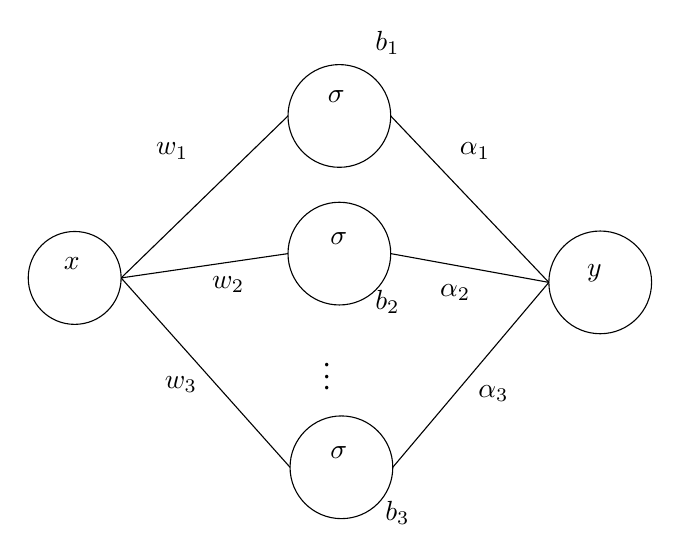
\begin{tikzpicture}[x=0.75pt,y=0.75pt,yscale=-1.2,xscale=1.2]
\draw   (120.7,148.65) .. controls (120.7,138.35) and (129.05,130) .. (139.35,130) .. controls (149.65,130) and (158,138.35) .. (158,148.65) .. controls (158,158.95) and (149.65,167.3) .. (139.35,167.3) .. controls (129.05,167.3) and (120.7,158.95) .. (120.7,148.65) -- cycle ;
\draw   (225,83.62) .. controls (225,72.23) and (234.23,63) .. (245.62,63) .. controls (257.01,63) and (266.24,72.23) .. (266.24,83.62) .. controls (266.24,95.01) and (257.01,104.24) .. (245.62,104.24) .. controls (234.23,104.24) and (225,95.01) .. (225,83.62) -- cycle ;
\draw   (225,138.89) .. controls (225,127.5) and (234.23,118.27) .. (245.62,118.27) .. controls (257.01,118.27) and (266.24,127.5) .. (266.24,138.89) .. controls (266.24,150.28) and (257.01,159.51) .. (245.62,159.51) .. controls (234.23,159.51) and (225,150.28) .. (225,138.89) -- cycle ;
\draw   (225.82,224.68) .. controls (225.82,213.29) and (235.06,204.06) .. (246.45,204.06) .. controls (257.84,204.06) and (267.07,213.29) .. (267.07,224.68) .. controls (267.07,236.07) and (257.84,245.3) .. (246.45,245.3) .. controls (235.06,245.3) and (225.82,236.07) .. (225.82,224.68) -- cycle ;
\draw   (329.73,150.44) .. controls (329.73,139.05) and (338.97,129.82) .. (350.36,129.82) .. controls (361.74,129.82) and (370.98,139.05) .. (370.98,150.44) .. controls (370.98,161.83) and (361.74,171.06) .. (350.36,171.06) .. controls (338.97,171.06) and (329.73,161.83) .. (329.73,150.44) -- cycle ;
\draw    (158,148.65) -- (225,83.62) ;
\draw    (158,148.65) -- (225,138.89) ;
\draw    (158,148.65) -- (225.82,224.68) ;
\draw    (266.24,83.62) -- (329.73,150.44) ;
\draw    (266.24,138.89) -- (329.73,150.44) ;
\draw    (267.07,224.68) -- (329.73,150.44) ;
\draw (134,139.4) node [anchor=north west][inner sep=0.75pt]    {$x$};
\draw (238,175.4) node [anchor=north west][inner sep=0.75pt]    {$\vdots $};
\draw (240,72.4) node [anchor=north west][inner sep=0.75pt]    {$\sigma $};
\draw (241,129.4) node [anchor=north west][inner sep=0.75pt]    {$\sigma $};
\draw (241,215.4) node [anchor=north west][inner sep=0.75pt]    {$\sigma $};
\draw (344,142.4) node [anchor=north west][inner sep=0.75pt]    {$y$};
\draw (171,93.4) node [anchor=north west][inner sep=0.75pt]    {$w_{1}$};
\draw (193.5,147.17) node [anchor=north west][inner sep=0.75pt]    {$w_{2}$};
\draw (174.5,187.17) node [anchor=north west][inner sep=0.75pt]    {$w_{3}$};
\draw (259,48.4) node [anchor=north west][inner sep=0.75pt]    {$b_{1}$};
\draw (259,152.4) node [anchor=north west][inner sep=0.75pt]    {$b_{2}$};
\draw (293,93.4) node [anchor=north west][inner sep=0.75pt]    {$\alpha _{1}$};
\draw (263,237.4) node [anchor=north west][inner sep=0.75pt]    {$b_{3}$};
\draw (285,150.4) node [anchor=north west][inner sep=0.75pt]    {$\alpha _{2}$};
\draw (300.4,190.96) node [anchor=north west][inner sep=0.75pt]    {$\alpha _{3}$};
\end{tikzpicture}
\end{center} \par 
More generally, the least square problem when $\mathcal{H}$ is nonlinear can be written as \begin{equation}\label{eq7} \min_\alpha\dfrac{1}{n}\sum_{i=1}^n\qty\Big(y_i-\underbrace{\phi(x_i;\alpha)}_\text{nonlinear})\end{equation}
As $\phi(x;\alpha)$ is nonlinear, we cannot write it as a matrix-vector product as given in (\ref{eq6}). \par 
(\ref{eq7}) is called a \textit{nonlinear least square problem}.
\begin{rmk}
	We obtain nonlinear least square problems when we fit data with square loss and nonlinear model. 
\end{rmk}

\begin{description}
	\item[Problem: Data Classification] Given $(x_1,y_1),\dots,(x_n,y_n)$, find $\phi(x;\alpha)\st\phi(x_i;\alpha)\approx y_i\quad\forall i$.
	\begin{center}
	\tikzset{every picture/.style={line width=0.75pt}}
	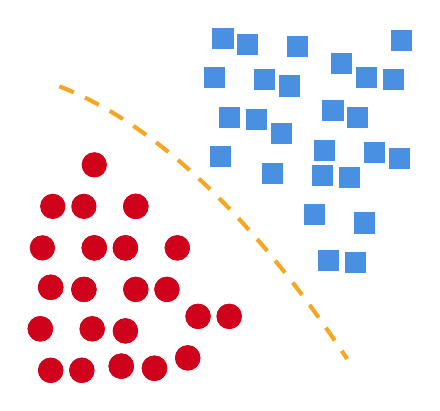
\begin{tikzpicture}[x=0.75pt,y=0.75pt,yscale=-1,xscale=1]
	\draw  [color={rgb, 255:red, 208; green, 2; blue, 27 }  ,draw opacity=1 ][fill={rgb, 255:red, 208; green, 2; blue, 27 }  ,fill opacity=1 ] (139,168.82) .. controls (139,165.61) and (141.61,163) .. (144.82,163) .. controls (148.04,163) and (150.65,165.61) .. (150.65,168.82) .. controls (150.65,172.04) and (148.04,174.65) .. (144.82,174.65) .. controls (141.61,174.65) and (139,172.04) .. (139,168.82) -- cycle ;
	\draw  [color={rgb, 255:red, 208; green, 2; blue, 27 }  ,draw opacity=1 ][fill={rgb, 255:red, 208; green, 2; blue, 27 }  ,fill opacity=1 ] (139,168.82) .. controls (139,165.61) and (141.61,163) .. (144.82,163) .. controls (148.04,163) and (150.65,165.61) .. (150.65,168.82) .. controls (150.65,172.04) and (148.04,174.65) .. (144.82,174.65) .. controls (141.61,174.65) and (139,172.04) .. (139,168.82) -- cycle ;
	\draw  [color={rgb, 255:red, 208; green, 2; blue, 27 }  ,draw opacity=1 ][fill={rgb, 255:red, 208; green, 2; blue, 27 }  ,fill opacity=1 ] (134,188.82) .. controls (134,185.61) and (136.61,183) .. (139.82,183) .. controls (143.04,183) and (145.65,185.61) .. (145.65,188.82) .. controls (145.65,192.04) and (143.04,194.65) .. (139.82,194.65) .. controls (136.61,194.65) and (134,192.04) .. (134,188.82) -- cycle ;
	\draw  [color={rgb, 255:red, 208; green, 2; blue, 27 }  ,draw opacity=1 ][fill={rgb, 255:red, 208; green, 2; blue, 27 }  ,fill opacity=1 ] (134,188.82) .. controls (134,185.61) and (136.61,183) .. (139.82,183) .. controls (143.04,183) and (145.65,185.61) .. (145.65,188.82) .. controls (145.65,192.04) and (143.04,194.65) .. (139.82,194.65) .. controls (136.61,194.65) and (134,192.04) .. (134,188.82) -- cycle ;
	\draw  [color={rgb, 255:red, 208; green, 2; blue, 27 }  ,draw opacity=1 ][fill={rgb, 255:red, 208; green, 2; blue, 27 }  ,fill opacity=1 ] (139,208.82) .. controls (139,205.61) and (141.61,203) .. (144.82,203) .. controls (148.04,203) and (150.65,205.61) .. (150.65,208.82) .. controls (150.65,212.04) and (148.04,214.65) .. (144.82,214.65) .. controls (141.61,214.65) and (139,212.04) .. (139,208.82) -- cycle ;
	\draw  [color={rgb, 255:red, 208; green, 2; blue, 27 }  ,draw opacity=1 ][fill={rgb, 255:red, 208; green, 2; blue, 27 }  ,fill opacity=1 ] (139,208.82) .. controls (139,205.61) and (141.61,203) .. (144.82,203) .. controls (148.04,203) and (150.65,205.61) .. (150.65,208.82) .. controls (150.65,212.04) and (148.04,214.65) .. (144.82,214.65) .. controls (141.61,214.65) and (139,212.04) .. (139,208.82) -- cycle ;
	\draw  [color={rgb, 255:red, 208; green, 2; blue, 27 }  ,draw opacity=1 ][fill={rgb, 255:red, 208; green, 2; blue, 27 }  ,fill opacity=1 ] (139,168.82) .. controls (139,165.61) and (141.61,163) .. (144.82,163) .. controls (148.04,163) and (150.65,165.61) .. (150.65,168.82) .. controls (150.65,172.04) and (148.04,174.65) .. (144.82,174.65) .. controls (141.61,174.65) and (139,172.04) .. (139,168.82) -- cycle ;
	\draw  [color={rgb, 255:red, 208; green, 2; blue, 27 }  ,draw opacity=1 ][fill={rgb, 255:red, 208; green, 2; blue, 27 }  ,fill opacity=1 ] (159,188.82) .. controls (159,185.61) and (161.61,183) .. (164.82,183) .. controls (168.04,183) and (170.65,185.61) .. (170.65,188.82) .. controls (170.65,192.04) and (168.04,194.65) .. (164.82,194.65) .. controls (161.61,194.65) and (159,192.04) .. (159,188.82) -- cycle ;
	\draw  [color={rgb, 255:red, 208; green, 2; blue, 27 }  ,draw opacity=1 ][fill={rgb, 255:red, 208; green, 2; blue, 27 }  ,fill opacity=1 ] (159,188.82) .. controls (159,185.61) and (161.61,183) .. (164.82,183) .. controls (168.04,183) and (170.65,185.61) .. (170.65,188.82) .. controls (170.65,192.04) and (168.04,194.65) .. (164.82,194.65) .. controls (161.61,194.65) and (159,192.04) .. (159,188.82) -- cycle ;
	\draw  [color={rgb, 255:red, 208; green, 2; blue, 27 }  ,draw opacity=1 ][fill={rgb, 255:red, 208; green, 2; blue, 27 }  ,fill opacity=1 ] (134,188.82) .. controls (134,185.61) and (136.61,183) .. (139.82,183) .. controls (143.04,183) and (145.65,185.61) .. (145.65,188.82) .. controls (145.65,192.04) and (143.04,194.65) .. (139.82,194.65) .. controls (136.61,194.65) and (134,192.04) .. (134,188.82) -- cycle ;
	\draw  [color={rgb, 255:red, 208; green, 2; blue, 27 }  ,draw opacity=1 ][fill={rgb, 255:red, 208; green, 2; blue, 27 }  ,fill opacity=1 ] (154,208.82) .. controls (154,205.61) and (156.61,203) .. (159.82,203) .. controls (163.04,203) and (165.65,205.61) .. (165.65,208.82) .. controls (165.65,212.04) and (163.04,214.65) .. (159.82,214.65) .. controls (156.61,214.65) and (154,212.04) .. (154,208.82) -- cycle ;
	\draw  [color={rgb, 255:red, 208; green, 2; blue, 27 }  ,draw opacity=1 ][fill={rgb, 255:red, 208; green, 2; blue, 27 }  ,fill opacity=1 ] (154,208.82) .. controls (154,205.61) and (156.61,203) .. (159.82,203) .. controls (163.04,203) and (165.65,205.61) .. (165.65,208.82) .. controls (165.65,212.04) and (163.04,214.65) .. (159.82,214.65) .. controls (156.61,214.65) and (154,212.04) .. (154,208.82) -- cycle ;
	\draw  [color={rgb, 255:red, 208; green, 2; blue, 27 }  ,draw opacity=1 ][fill={rgb, 255:red, 208; green, 2; blue, 27 }  ,fill opacity=1 ] (140,129.82) .. controls (140,126.61) and (142.61,124) .. (145.82,124) .. controls (149.04,124) and (151.65,126.61) .. (151.65,129.82) .. controls (151.65,133.04) and (149.04,135.65) .. (145.82,135.65) .. controls (142.61,135.65) and (140,133.04) .. (140,129.82) -- cycle ;
	\draw  [color={rgb, 255:red, 208; green, 2; blue, 27 }  ,draw opacity=1 ][fill={rgb, 255:red, 208; green, 2; blue, 27 }  ,fill opacity=1 ] (160,149.82) .. controls (160,146.61) and (162.61,144) .. (165.82,144) .. controls (169.04,144) and (171.65,146.61) .. (171.65,149.82) .. controls (171.65,153.04) and (169.04,155.65) .. (165.82,155.65) .. controls (162.61,155.65) and (160,153.04) .. (160,149.82) -- cycle ;
	\draw  [color={rgb, 255:red, 208; green, 2; blue, 27 }  ,draw opacity=1 ][fill={rgb, 255:red, 208; green, 2; blue, 27 }  ,fill opacity=1 ] (160,149.82) .. controls (160,146.61) and (162.61,144) .. (165.82,144) .. controls (169.04,144) and (171.65,146.61) .. (171.65,149.82) .. controls (171.65,153.04) and (169.04,155.65) .. (165.82,155.65) .. controls (162.61,155.65) and (160,153.04) .. (160,149.82) -- cycle ;
	\draw  [color={rgb, 255:red, 208; green, 2; blue, 27 }  ,draw opacity=1 ][fill={rgb, 255:red, 208; green, 2; blue, 27 }  ,fill opacity=1 ] (135,149.82) .. controls (135,146.61) and (137.61,144) .. (140.82,144) .. controls (144.04,144) and (146.65,146.61) .. (146.65,149.82) .. controls (146.65,153.04) and (144.04,155.65) .. (140.82,155.65) .. controls (137.61,155.65) and (135,153.04) .. (135,149.82) -- cycle ;
	\draw  [color={rgb, 255:red, 208; green, 2; blue, 27 }  ,draw opacity=1 ][fill={rgb, 255:red, 208; green, 2; blue, 27 }  ,fill opacity=1 ] (155,169.82) .. controls (155,166.61) and (157.61,164) .. (160.82,164) .. controls (164.04,164) and (166.65,166.61) .. (166.65,169.82) .. controls (166.65,173.04) and (164.04,175.65) .. (160.82,175.65) .. controls (157.61,175.65) and (155,173.04) .. (155,169.82) -- cycle ;
	\draw  [color={rgb, 255:red, 208; green, 2; blue, 27 }  ,draw opacity=1 ][fill={rgb, 255:red, 208; green, 2; blue, 27 }  ,fill opacity=1 ] (155,169.82) .. controls (155,166.61) and (157.61,164) .. (160.82,164) .. controls (164.04,164) and (166.65,166.61) .. (166.65,169.82) .. controls (166.65,173.04) and (164.04,175.65) .. (160.82,175.65) .. controls (157.61,175.65) and (155,173.04) .. (155,169.82) -- cycle ;
	\draw  [color={rgb, 255:red, 208; green, 2; blue, 27 }  ,draw opacity=1 ][fill={rgb, 255:red, 208; green, 2; blue, 27 }  ,fill opacity=1 ] (160,109.82) .. controls (160,106.61) and (162.61,104) .. (165.82,104) .. controls (169.04,104) and (171.65,106.61) .. (171.65,109.82) .. controls (171.65,113.04) and (169.04,115.65) .. (165.82,115.65) .. controls (162.61,115.65) and (160,113.04) .. (160,109.82) -- cycle ;
	\draw  [color={rgb, 255:red, 208; green, 2; blue, 27 }  ,draw opacity=1 ][fill={rgb, 255:red, 208; green, 2; blue, 27 }  ,fill opacity=1 ] (180,129.82) .. controls (180,126.61) and (182.61,124) .. (185.82,124) .. controls (189.04,124) and (191.65,126.61) .. (191.65,129.82) .. controls (191.65,133.04) and (189.04,135.65) .. (185.82,135.65) .. controls (182.61,135.65) and (180,133.04) .. (180,129.82) -- cycle ;
	\draw  [color={rgb, 255:red, 208; green, 2; blue, 27 }  ,draw opacity=1 ][fill={rgb, 255:red, 208; green, 2; blue, 27 }  ,fill opacity=1 ] (180,129.82) .. controls (180,126.61) and (182.61,124) .. (185.82,124) .. controls (189.04,124) and (191.65,126.61) .. (191.65,129.82) .. controls (191.65,133.04) and (189.04,135.65) .. (185.82,135.65) .. controls (182.61,135.65) and (180,133.04) .. (180,129.82) -- cycle ;
	\draw  [color={rgb, 255:red, 208; green, 2; blue, 27 }  ,draw opacity=1 ][fill={rgb, 255:red, 208; green, 2; blue, 27 }  ,fill opacity=1 ] (155,129.82) .. controls (155,126.61) and (157.61,124) .. (160.82,124) .. controls (164.04,124) and (166.65,126.61) .. (166.65,129.82) .. controls (166.65,133.04) and (164.04,135.65) .. (160.82,135.65) .. controls (157.61,135.65) and (155,133.04) .. (155,129.82) -- cycle ;
	\draw  [color={rgb, 255:red, 208; green, 2; blue, 27 }  ,draw opacity=1 ][fill={rgb, 255:red, 208; green, 2; blue, 27 }  ,fill opacity=1 ] (175,149.82) .. controls (175,146.61) and (177.61,144) .. (180.82,144) .. controls (184.04,144) and (186.65,146.61) .. (186.65,149.82) .. controls (186.65,153.04) and (184.04,155.65) .. (180.82,155.65) .. controls (177.61,155.65) and (175,153.04) .. (175,149.82) -- cycle ;
	\draw  [color={rgb, 255:red, 208; green, 2; blue, 27 }  ,draw opacity=1 ][fill={rgb, 255:red, 208; green, 2; blue, 27 }  ,fill opacity=1 ] (175,149.82) .. controls (175,146.61) and (177.61,144) .. (180.82,144) .. controls (184.04,144) and (186.65,146.61) .. (186.65,149.82) .. controls (186.65,153.04) and (184.04,155.65) .. (180.82,155.65) .. controls (177.61,155.65) and (175,153.04) .. (175,149.82) -- cycle ;
	\draw  [color={rgb, 255:red, 208; green, 2; blue, 27 }  ,draw opacity=1 ][fill={rgb, 255:red, 208; green, 2; blue, 27 }  ,fill opacity=1 ] (160,149.82) .. controls (160,146.61) and (162.61,144) .. (165.82,144) .. controls (169.04,144) and (171.65,146.61) .. (171.65,149.82) .. controls (171.65,153.04) and (169.04,155.65) .. (165.82,155.65) .. controls (162.61,155.65) and (160,153.04) .. (160,149.82) -- cycle ;
	\draw  [color={rgb, 255:red, 208; green, 2; blue, 27 }  ,draw opacity=1 ][fill={rgb, 255:red, 208; green, 2; blue, 27 }  ,fill opacity=1 ] (180,169.82) .. controls (180,166.61) and (182.61,164) .. (185.82,164) .. controls (189.04,164) and (191.65,166.61) .. (191.65,169.82) .. controls (191.65,173.04) and (189.04,175.65) .. (185.82,175.65) .. controls (182.61,175.65) and (180,173.04) .. (180,169.82) -- cycle ;
	\draw  [color={rgb, 255:red, 208; green, 2; blue, 27 }  ,draw opacity=1 ][fill={rgb, 255:red, 208; green, 2; blue, 27 }  ,fill opacity=1 ] (180,169.82) .. controls (180,166.61) and (182.61,164) .. (185.82,164) .. controls (189.04,164) and (191.65,166.61) .. (191.65,169.82) .. controls (191.65,173.04) and (189.04,175.65) .. (185.82,175.65) .. controls (182.61,175.65) and (180,173.04) .. (180,169.82) -- cycle ;
	\draw  [color={rgb, 255:red, 208; green, 2; blue, 27 }  ,draw opacity=1 ][fill={rgb, 255:red, 208; green, 2; blue, 27 }  ,fill opacity=1 ] (155,169.82) .. controls (155,166.61) and (157.61,164) .. (160.82,164) .. controls (164.04,164) and (166.65,166.61) .. (166.65,169.82) .. controls (166.65,173.04) and (164.04,175.65) .. (160.82,175.65) .. controls (157.61,175.65) and (155,173.04) .. (155,169.82) -- cycle ;
	\draw  [color={rgb, 255:red, 208; green, 2; blue, 27 }  ,draw opacity=1 ][fill={rgb, 255:red, 208; green, 2; blue, 27 }  ,fill opacity=1 ] (175,189.82) .. controls (175,186.61) and (177.61,184) .. (180.82,184) .. controls (184.04,184) and (186.65,186.61) .. (186.65,189.82) .. controls (186.65,193.04) and (184.04,195.65) .. (180.82,195.65) .. controls (177.61,195.65) and (175,193.04) .. (175,189.82) -- cycle ;
	\draw  [color={rgb, 255:red, 208; green, 2; blue, 27 }  ,draw opacity=1 ][fill={rgb, 255:red, 208; green, 2; blue, 27 }  ,fill opacity=1 ] (175,189.82) .. controls (175,186.61) and (177.61,184) .. (180.82,184) .. controls (184.04,184) and (186.65,186.61) .. (186.65,189.82) .. controls (186.65,193.04) and (184.04,195.65) .. (180.82,195.65) .. controls (177.61,195.65) and (175,193.04) .. (175,189.82) -- cycle ;
	\draw  [color={rgb, 255:red, 208; green, 2; blue, 27 }  ,draw opacity=1 ][fill={rgb, 255:red, 208; green, 2; blue, 27 }  ,fill opacity=1 ] (180,129.82) .. controls (180,126.61) and (182.61,124) .. (185.82,124) .. controls (189.04,124) and (191.65,126.61) .. (191.65,129.82) .. controls (191.65,133.04) and (189.04,135.65) .. (185.82,135.65) .. controls (182.61,135.65) and (180,133.04) .. (180,129.82) -- cycle ;
	\draw  [color={rgb, 255:red, 208; green, 2; blue, 27 }  ,draw opacity=1 ][fill={rgb, 255:red, 208; green, 2; blue, 27 }  ,fill opacity=1 ] (200,149.82) .. controls (200,146.61) and (202.61,144) .. (205.82,144) .. controls (209.04,144) and (211.65,146.61) .. (211.65,149.82) .. controls (211.65,153.04) and (209.04,155.65) .. (205.82,155.65) .. controls (202.61,155.65) and (200,153.04) .. (200,149.82) -- cycle ;
	\draw  [color={rgb, 255:red, 208; green, 2; blue, 27 }  ,draw opacity=1 ][fill={rgb, 255:red, 208; green, 2; blue, 27 }  ,fill opacity=1 ] (200,149.82) .. controls (200,146.61) and (202.61,144) .. (205.82,144) .. controls (209.04,144) and (211.65,146.61) .. (211.65,149.82) .. controls (211.65,153.04) and (209.04,155.65) .. (205.82,155.65) .. controls (202.61,155.65) and (200,153.04) .. (200,149.82) -- cycle ;
	\draw  [color={rgb, 255:red, 208; green, 2; blue, 27 }  ,draw opacity=1 ][fill={rgb, 255:red, 208; green, 2; blue, 27 }  ,fill opacity=1 ] (175,149.82) .. controls (175,146.61) and (177.61,144) .. (180.82,144) .. controls (184.04,144) and (186.65,146.61) .. (186.65,149.82) .. controls (186.65,153.04) and (184.04,155.65) .. (180.82,155.65) .. controls (177.61,155.65) and (175,153.04) .. (175,149.82) -- cycle ;
	\draw  [color={rgb, 255:red, 208; green, 2; blue, 27 }  ,draw opacity=1 ][fill={rgb, 255:red, 208; green, 2; blue, 27 }  ,fill opacity=1 ] (195,169.82) .. controls (195,166.61) and (197.61,164) .. (200.82,164) .. controls (204.04,164) and (206.65,166.61) .. (206.65,169.82) .. controls (206.65,173.04) and (204.04,175.65) .. (200.82,175.65) .. controls (197.61,175.65) and (195,173.04) .. (195,169.82) -- cycle ;
	\draw  [color={rgb, 255:red, 208; green, 2; blue, 27 }  ,draw opacity=1 ][fill={rgb, 255:red, 208; green, 2; blue, 27 }  ,fill opacity=1 ] (195,169.82) .. controls (195,166.61) and (197.61,164) .. (200.82,164) .. controls (204.04,164) and (206.65,166.61) .. (206.65,169.82) .. controls (206.65,173.04) and (204.04,175.65) .. (200.82,175.65) .. controls (197.61,175.65) and (195,173.04) .. (195,169.82) -- cycle ;
	\draw  [color={rgb, 255:red, 208; green, 2; blue, 27 }  ,draw opacity=1 ][fill={rgb, 255:red, 208; green, 2; blue, 27 }  ,fill opacity=1 ] (173,206.82) .. controls (173,203.61) and (175.61,201) .. (178.82,201) .. controls (182.04,201) and (184.65,203.61) .. (184.65,206.82) .. controls (184.65,210.04) and (182.04,212.65) .. (178.82,212.65) .. controls (175.61,212.65) and (173,210.04) .. (173,206.82) -- cycle ;
	\draw  [color={rgb, 255:red, 208; green, 2; blue, 27 }  ,draw opacity=1 ][fill={rgb, 255:red, 208; green, 2; blue, 27 }  ,fill opacity=1 ] (173,206.82) .. controls (173,203.61) and (175.61,201) .. (178.82,201) .. controls (182.04,201) and (184.65,203.61) .. (184.65,206.82) .. controls (184.65,210.04) and (182.04,212.65) .. (178.82,212.65) .. controls (175.61,212.65) and (173,210.04) .. (173,206.82) -- cycle ;
	\draw  [color={rgb, 255:red, 208; green, 2; blue, 27 }  ,draw opacity=1 ][fill={rgb, 255:red, 208; green, 2; blue, 27 }  ,fill opacity=1 ] (173,206.82) .. controls (173,203.61) and (175.61,201) .. (178.82,201) .. controls (182.04,201) and (184.65,203.61) .. (184.65,206.82) .. controls (184.65,210.04) and (182.04,212.65) .. (178.82,212.65) .. controls (175.61,212.65) and (173,210.04) .. (173,206.82) -- cycle ;
	\draw  [color={rgb, 255:red, 208; green, 2; blue, 27 }  ,draw opacity=1 ][fill={rgb, 255:red, 208; green, 2; blue, 27 }  ,fill opacity=1 ] (189,207.82) .. controls (189,204.61) and (191.61,202) .. (194.82,202) .. controls (198.04,202) and (200.65,204.61) .. (200.65,207.82) .. controls (200.65,211.04) and (198.04,213.65) .. (194.82,213.65) .. controls (191.61,213.65) and (189,211.04) .. (189,207.82) -- cycle ;
	\draw  [color={rgb, 255:red, 208; green, 2; blue, 27 }  ,draw opacity=1 ][fill={rgb, 255:red, 208; green, 2; blue, 27 }  ,fill opacity=1 ] (189,207.82) .. controls (189,204.61) and (191.61,202) .. (194.82,202) .. controls (198.04,202) and (200.65,204.61) .. (200.65,207.82) .. controls (200.65,211.04) and (198.04,213.65) .. (194.82,213.65) .. controls (191.61,213.65) and (189,211.04) .. (189,207.82) -- cycle ;
	\draw  [color={rgb, 255:red, 208; green, 2; blue, 27 }  ,draw opacity=1 ][fill={rgb, 255:red, 208; green, 2; blue, 27 }  ,fill opacity=1 ] (210,182.82) .. controls (210,179.61) and (212.61,177) .. (215.82,177) .. controls (219.04,177) and (221.65,179.61) .. (221.65,182.82) .. controls (221.65,186.04) and (219.04,188.65) .. (215.82,188.65) .. controls (212.61,188.65) and (210,186.04) .. (210,182.82) -- cycle ;
	\draw  [color={rgb, 255:red, 208; green, 2; blue, 27 }  ,draw opacity=1 ][fill={rgb, 255:red, 208; green, 2; blue, 27 }  ,fill opacity=1 ] (210,182.82) .. controls (210,179.61) and (212.61,177) .. (215.82,177) .. controls (219.04,177) and (221.65,179.61) .. (221.65,182.82) .. controls (221.65,186.04) and (219.04,188.65) .. (215.82,188.65) .. controls (212.61,188.65) and (210,186.04) .. (210,182.82) -- cycle ;
	\draw  [color={rgb, 255:red, 208; green, 2; blue, 27 }  ,draw opacity=1 ][fill={rgb, 255:red, 208; green, 2; blue, 27 }  ,fill opacity=1 ] (189,207.82) .. controls (189,204.61) and (191.61,202) .. (194.82,202) .. controls (198.04,202) and (200.65,204.61) .. (200.65,207.82) .. controls (200.65,211.04) and (198.04,213.65) .. (194.82,213.65) .. controls (191.61,213.65) and (189,211.04) .. (189,207.82) -- cycle ;
	\draw  [color={rgb, 255:red, 208; green, 2; blue, 27 }  ,draw opacity=1 ][fill={rgb, 255:red, 208; green, 2; blue, 27 }  ,fill opacity=1 ] (205,202.82) .. controls (205,199.61) and (207.61,197) .. (210.82,197) .. controls (214.04,197) and (216.65,199.61) .. (216.65,202.82) .. controls (216.65,206.04) and (214.04,208.65) .. (210.82,208.65) .. controls (207.61,208.65) and (205,206.04) .. (205,202.82) -- cycle ;
	\draw  [color={rgb, 255:red, 208; green, 2; blue, 27 }  ,draw opacity=1 ][fill={rgb, 255:red, 208; green, 2; blue, 27 }  ,fill opacity=1 ] (205,202.82) .. controls (205,199.61) and (207.61,197) .. (210.82,197) .. controls (214.04,197) and (216.65,199.61) .. (216.65,202.82) .. controls (216.65,206.04) and (214.04,208.65) .. (210.82,208.65) .. controls (207.61,208.65) and (205,206.04) .. (205,202.82) -- cycle ;
	\draw  [color={rgb, 255:red, 208; green, 2; blue, 27 }  ,draw opacity=1 ][fill={rgb, 255:red, 208; green, 2; blue, 27 }  ,fill opacity=1 ] (225,182.82) .. controls (225,179.61) and (227.61,177) .. (230.82,177) .. controls (234.04,177) and (236.65,179.61) .. (236.65,182.82) .. controls (236.65,186.04) and (234.04,188.65) .. (230.82,188.65) .. controls (227.61,188.65) and (225,186.04) .. (225,182.82) -- cycle ;
	\draw  [color={rgb, 255:red, 208; green, 2; blue, 27 }  ,draw opacity=1 ][fill={rgb, 255:red, 208; green, 2; blue, 27 }  ,fill opacity=1 ] (225,182.82) .. controls (225,179.61) and (227.61,177) .. (230.82,177) .. controls (234.04,177) and (236.65,179.61) .. (236.65,182.82) .. controls (236.65,186.04) and (234.04,188.65) .. (230.82,188.65) .. controls (227.61,188.65) and (225,186.04) .. (225,182.82) -- cycle ;
	\draw  [color={rgb, 255:red, 74; green, 144; blue, 226 }  ,draw opacity=1 ][fill={rgb, 255:red, 74; green, 144; blue, 226 }  ,fill opacity=1 ] (292,63) -- (301.65,63) -- (301.65,72.65) -- (292,72.65) -- cycle ;
	\draw  [color={rgb, 255:red, 74; green, 144; blue, 226 }  ,draw opacity=1 ][fill={rgb, 255:red, 74; green, 144; blue, 226 }  ,fill opacity=1 ] (274,151) -- (283.65,151) -- (283.65,160.65) -- (274,160.65) -- cycle ;
	\draw  [color={rgb, 255:red, 74; green, 144; blue, 226 }  ,draw opacity=1 ][fill={rgb, 255:red, 74; green, 144; blue, 226 }  ,fill opacity=1 ] (288,82) -- (297.65,82) -- (297.65,91.65) -- (288,91.65) -- cycle ;
	\draw  [color={rgb, 255:red, 74; green, 144; blue, 226 }  ,draw opacity=1 ][fill={rgb, 255:red, 74; green, 144; blue, 226 }  ,fill opacity=1 ] (308,102) -- (317.65,102) -- (317.65,111.65) -- (308,111.65) -- cycle ;
	\draw  [color={rgb, 255:red, 74; green, 144; blue, 226 }  ,draw opacity=1 ][fill={rgb, 255:red, 74; green, 144; blue, 226 }  ,fill opacity=1 ] (309,45) -- (318.65,45) -- (318.65,54.65) -- (309,54.65) -- cycle ;
	\draw  [color={rgb, 255:red, 74; green, 144; blue, 226 }  ,draw opacity=1 ][fill={rgb, 255:red, 74; green, 144; blue, 226 }  ,fill opacity=1 ] (291,133) -- (300.65,133) -- (300.65,142.65) -- (291,142.65) -- cycle ;
	\draw  [color={rgb, 255:red, 74; green, 144; blue, 226 }  ,draw opacity=1 ][fill={rgb, 255:red, 74; green, 144; blue, 226 }  ,fill opacity=1 ] (305,64) -- (314.65,64) -- (314.65,73.65) -- (305,73.65) -- cycle ;
	\draw  [color={rgb, 255:red, 74; green, 144; blue, 226 }  ,draw opacity=1 ][fill={rgb, 255:red, 74; green, 144; blue, 226 }  ,fill opacity=1 ] (287,152) -- (296.65,152) -- (296.65,161.65) -- (287,161.65) -- cycle ;
	\draw  [color={rgb, 255:red, 74; green, 144; blue, 226 }  ,draw opacity=1 ][fill={rgb, 255:red, 74; green, 144; blue, 226 }  ,fill opacity=1 ] (251,90) -- (260.65,90) -- (260.65,99.65) -- (251,99.65) -- cycle ;
	\draw  [color={rgb, 255:red, 74; green, 144; blue, 226 }  ,draw opacity=1 ][fill={rgb, 255:red, 74; green, 144; blue, 226 }  ,fill opacity=1 ] (271,110) -- (280.65,110) -- (280.65,119.65) -- (271,119.65) -- cycle ;
	\draw  [color={rgb, 255:red, 74; green, 144; blue, 226 }  ,draw opacity=1 ][fill={rgb, 255:red, 74; green, 144; blue, 226 }  ,fill opacity=1 ] (247,109) -- (256.65,109) -- (256.65,118.65) -- (247,118.65) -- cycle ;
	\draw  [color={rgb, 255:red, 74; green, 144; blue, 226 }  ,draw opacity=1 ][fill={rgb, 255:red, 74; green, 144; blue, 226 }  ,fill opacity=1 ] (267,129) -- (276.65,129) -- (276.65,138.65) -- (267,138.65) -- cycle ;
	\draw  [color={rgb, 255:red, 74; green, 144; blue, 226 }  ,draw opacity=1 ][fill={rgb, 255:red, 74; green, 144; blue, 226 }  ,fill opacity=1 ] (276,79) -- (285.65,79) -- (285.65,88.65) -- (276,88.65) -- cycle ;
	\draw  [color={rgb, 255:red, 74; green, 144; blue, 226 }  ,draw opacity=1 ][fill={rgb, 255:red, 74; green, 144; blue, 226 }  ,fill opacity=1 ] (296,99) -- (305.65,99) -- (305.65,108.65) -- (296,108.65) -- cycle ;
	\draw  [color={rgb, 255:red, 74; green, 144; blue, 226 }  ,draw opacity=1 ][fill={rgb, 255:red, 74; green, 144; blue, 226 }  ,fill opacity=1 ] (272,98) -- (281.65,98) -- (281.65,107.65) -- (272,107.65) -- cycle ;
	\draw  [color={rgb, 255:red, 74; green, 144; blue, 226 }  ,draw opacity=1 ][fill={rgb, 255:red, 74; green, 144; blue, 226 }  ,fill opacity=1 ] (284,111) -- (293.65,111) -- (293.65,120.65) -- (284,120.65) -- cycle ;
	\draw  [color={rgb, 255:red, 74; green, 144; blue, 226 }  ,draw opacity=1 ][fill={rgb, 255:red, 74; green, 144; blue, 226 }  ,fill opacity=1 ] (259,48) -- (268.65,48) -- (268.65,57.65) -- (259,57.65) -- cycle ;
	\draw  [color={rgb, 255:red, 74; green, 144; blue, 226 }  ,draw opacity=1 ][fill={rgb, 255:red, 74; green, 144; blue, 226 }  ,fill opacity=1 ] (235,47) -- (244.65,47) -- (244.65,56.65) -- (235,56.65) -- cycle ;
	\draw  [color={rgb, 255:red, 74; green, 144; blue, 226 }  ,draw opacity=1 ][fill={rgb, 255:red, 74; green, 144; blue, 226 }  ,fill opacity=1 ] (255,67) -- (264.65,67) -- (264.65,76.65) -- (255,76.65) -- cycle ;
	\draw  [color={rgb, 255:red, 74; green, 144; blue, 226 }  ,draw opacity=1 ][fill={rgb, 255:red, 74; green, 144; blue, 226 }  ,fill opacity=1 ] (280,56) -- (289.65,56) -- (289.65,65.65) -- (280,65.65) -- cycle ;
	\draw  [color={rgb, 255:red, 74; green, 144; blue, 226 }  ,draw opacity=1 ][fill={rgb, 255:red, 74; green, 144; blue, 226 }  ,fill opacity=1 ] (226,82) -- (235.65,82) -- (235.65,91.65) -- (226,91.65) -- cycle ;
	\draw  [color={rgb, 255:red, 74; green, 144; blue, 226 }  ,draw opacity=1 ][fill={rgb, 255:red, 74; green, 144; blue, 226 }  ,fill opacity=1 ] (222,101) -- (231.65,101) -- (231.65,110.65) -- (222,110.65) -- cycle ;
	\draw  [color={rgb, 255:red, 74; green, 144; blue, 226 }  ,draw opacity=1 ][fill={rgb, 255:red, 74; green, 144; blue, 226 }  ,fill opacity=1 ] (223,44) -- (232.65,44) -- (232.65,53.65) -- (223,53.65) -- cycle ;
	\draw  [color={rgb, 255:red, 74; green, 144; blue, 226 }  ,draw opacity=1 ][fill={rgb, 255:red, 74; green, 144; blue, 226 }  ,fill opacity=1 ] (243,64) -- (252.65,64) -- (252.65,73.65) -- (243,73.65) -- cycle ;
	\draw  [color={rgb, 255:red, 74; green, 144; blue, 226 }  ,draw opacity=1 ][fill={rgb, 255:red, 74; green, 144; blue, 226 }  ,fill opacity=1 ] (219,63) -- (228.65,63) -- (228.65,72.65) -- (219,72.65) -- cycle ;
	\draw  [color={rgb, 255:red, 74; green, 144; blue, 226 }  ,draw opacity=1 ][fill={rgb, 255:red, 74; green, 144; blue, 226 }  ,fill opacity=1 ] (239,83) -- (248.65,83) -- (248.65,92.65) -- (239,92.65) -- cycle ;
	\draw [color={rgb, 255:red, 245; green, 166; blue, 35 }  ,draw opacity=1 ][line width=1.5]  [dash pattern={on 5.63pt off 4.5pt}]  (149,72) .. controls (216.65,98.3) and (269.65,176.3) .. (287.65,203.3) ;
	\end{tikzpicture}
	\end{center}
	\item[Measuring Error:] What does $\phi(x;\alpha)\approx y_i$ mean?
		\begin{itemize}
			\item Distance -- MSE: $\dfrac{1}{n}\dsst\sum_{i=1}^n\qty(y_i-\phi(x;\alpha))^2$. Or, more generally, $\dfrac{1}{n}\dsst\sum_{i=1}^n\qty|y_i-\phi(x_i;\alpha)|^p$.
			\item Sign: $\dfrac{1}{n}\dsst\sum_{i=1}^n\qty(y_i-\operatorname{sign}(\phi(x_i;\alpha)))^2$, where \[\operatorname{sign}(x)=\begin{cases}1, &x>0\\0, &x=0\\-1, &x<0.\end{cases}\]
			\item \textit{Alternatively, $\operatorname{softmax}$, then the output will be $\phi(x;\alpha)\in\R^n$, where $n$ is the number of classes, with $\phi_i(x;\alpha)$ is the probability of $x$ in class $i$. For example, take $n=2$, then \[\phi(x;\alpha)=\qty(\phi_1(x;\alpha), \phi_2(x;\alpha))\] where $(1,0)$ means $100\%$ in class $1$ and $(0,1)$ means $100\%$ in class $2$. Turning everything into positive and probability values, we get \[\qty(\dfrac{e^{\phi_1(x;\alpha)}}{e^{\phi_1(x;\alpha)}+e^{\phi_2(x;\alpha)}},\dfrac{e^{\phi_2(x;\alpha)}}{e^{\phi_1(x;\alpha)}+e^{\phi_2(x;\alpha)}}).\]}
		\end{itemize}
	\item [Linear Least Square to Solve:] Suppose there exists some lines dividing the classes. Those lines are called hyperplanes with equation \[w\cdot x+\nu=0.\]
	\item[Goal] Find $w,\nu$ such that $w\cdot x+\nu>0$ for $x_i$ in {\color{red}{red}} and $w\cdot x+\nu<0$ for $x_i$ in {\color{blue}{blue}}. \par 
	\textit{However, we can have multiple choices of the hyperplane. Which one is better? We will evaluate them using the concept of \emph{margin}.}
	\begin{df}{Margin}
		We define the margin of the hyperplane defined by $w\cdot x+\nu=0$ as follows \[\rho(w)=\min_i\dfrac{\abs{w\cdot w_i+\nu}}{\norm{w}}.\]
	\end{df}
	If the classification is successful, we should have $w\cdot x_i+\nu$ and $y_i$ to have the same sign, so $\qty(w\cdot x_i+\nu)\cdot y_i\geq0$. Therefore, we want the hyperplane that \begin{align*}\max_{\qty(w\cdot x_i+\nu)\cdot y_i\geq0}\rho(w)&=\max_{\qty(w\cdot x_i+\nu)\cdot y_i\geq0}\min_i\dfrac{\abs{w\cdot w_i+\nu}}{\norm{w}}\\&=\max_{\qty(w\cdot x_i+\nu)\cdot y_i\geq0}\dfrac{1}{\norm{w}}&\text{by homogeneity of }w\text{ and }\nu\end{align*}
	We can further show that the optimization problem can be written as the following least square problem with respect to $w$ and $\nu$: \begin{equation}\label{eq8}\min_{\qty(w\cdot x_i+\nu)\cdot y_i\geq0}\dfrac{\norm{w}^2}{2}.\end{equation}
	\begin{prf} 
		In this proof, let's get a sense why we are having a least square problem. Suppose $w\in\R^{d\times1}$. Define \[A=\left(\begin{array}{c|c}\mqty{1&&0\\&\ddots&\\0&&1}&0\\\hline\\0&0\end{array}\right)=\mqty(I_d&0\\0&0).\] Then, \[A\mqty(w\\\nu)=\mqty(I_d&0\\0&0)\mqty(w\\\nu)=\mqty(w\\0),\quad b=\mqty(0_d\\0).\] Therefore, we get \[A\mqty(w\\\nu)-b=\mqty(w\\0)\implies\norm{A\mqty(w\\\nu)-b}^2=\norm{\mqty(w\\0)}=\norm{w}^2.\]
	\end{prf}
	\item[Nonlinear Least Square to Solve] We can form the following nonlinear least square problem \begin{equation}\label{eq9}\min_{w,\nu}\dfrac{1}{n}\sum_{i=1}^n\qty(y_i-\operatorname{sign}(w\cdot x_i+\nu))^2+\lambda_1\norm{w}^2+\lambda_2\norm{\nu}^2\end{equation} This is a nonlinear least square because $\operatorname{sign}(w\cdot _i+\nu)$ does not form a linear relationship with $w$ and $\nu$. This nonlinear least square will fail, in fact. To ensure \eqref{eq9} works, we have to add the constrain $(w\cdot x_i+\nu)\cdot y_i\geq1$.
	\item[Nonlinearly Separable Classification] If the classes are not linearly separable, neither \eqref{eq8} nor \eqref{eq9} will work. We need to transform them into a higher dimension. For example, consider the following mapping: $(x,y)\mapsto(x,y,x^2+y^2)$. The map that makes data linearly separable is the \textit{feature mapping}. Find a feature mapping can be very difficult. 
\end{description}

\newpage
\section{Constrained Optimization}
\begin{description}
	\item[Goal:] Constrained Optimal Problem
	\begin{itemize}
		\item figure out necessary conditions for optimality
		\item figure out sufficient conditions for optimality
		\item existence
		\item \texttt{MATLAB} function \texttt{fmincon}
	\end{itemize}
	\item[We will mostly discuss:] $\dsst\min_{x\in C}f(x)$, where$C$ is closed and convex, and $f$ can be either convex or non-convex. 
\end{description}
\subsection{Convexity}
\begin{df}{Convex Set}
	A set $C\subseteq\R^d$ is \textit{convex} if $\forall\ x,y\in C$ and $\lambda\in(0,1)$, we have that $(1-\lambda)x+\lambda y\in C$.
	\begin{rmk}
		Convexity essentially means that if we know two points are in the set, then everything on the line connecting the two points is also in the set. 	
	\end{rmk}
	\begin{center}
	\tikzset{every picture/.style={line width=0.75pt}}
	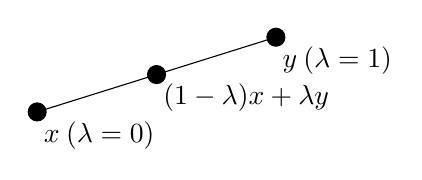
\begin{tikzpicture}[x=0.75pt,y=0.75pt,yscale=-1,xscale=1]
	\draw  [fill={rgb, 255:red, 0; green, 0; blue, 0 }  ,fill opacity=1 ] (100,125.32) .. controls (100,122.94) and (101.94,121) .. (104.32,121) .. controls (106.71,121) and (108.65,122.94) .. (108.65,125.32) .. controls (108.65,127.71) and (106.71,129.65) .. (104.32,129.65) .. controls (101.94,129.65) and (100,127.71) .. (100,125.32) -- cycle ;
	\draw  [fill={rgb, 255:red, 0; green, 0; blue, 0 }  ,fill opacity=1 ] (215,89.32) .. controls (215,86.94) and (216.94,85) .. (219.32,85) .. controls (221.71,85) and (223.65,86.94) .. (223.65,89.32) .. controls (223.65,91.71) and (221.71,93.65) .. (219.32,93.65) .. controls (216.94,93.65) and (215,91.71) .. (215,89.32) -- cycle ;
	\draw    (104.32,125.32) -- (219.32,89.32) ;
	\draw  [fill={rgb, 255:red, 0; green, 0; blue, 0 }  ,fill opacity=1 ] (157.5,107.32) .. controls (157.5,104.94) and (159.44,103) .. (161.82,103) .. controls (164.21,103) and (166.15,104.94) .. (166.15,107.32) .. controls (166.15,109.71) and (164.21,111.65) .. (161.82,111.65) .. controls (159.44,111.65) and (157.5,109.71) .. (157.5,107.32) -- cycle ;
	\draw (106.32,128.72) node [anchor=north west][inner sep=0.75pt]    {$x\ ( \lambda =0)$};
	\draw (221.32,92.72) node [anchor=north west][inner sep=0.75pt]    {$y\ ( \lambda =1)$};
	\draw (163.82,110.72) node [anchor=north west][inner sep=0.75pt]    {$( 1-\lambda ) x+\lambda y$};
	\end{tikzpicture}
	\end{center}
\end{df}
\begin{eg}{Example of convex and non-convex sets}
	\begin{center}
	\tikzset{every picture/.style={line width=0.75pt}}
	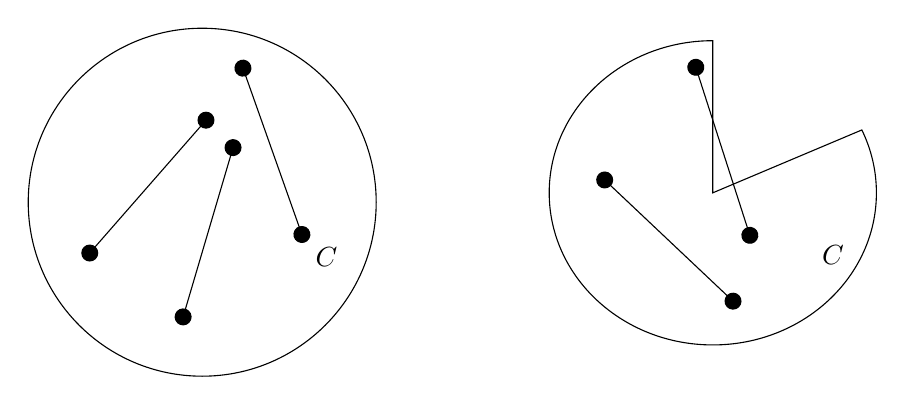
\begin{tikzpicture}[x=0.75pt,y=0.75pt,yscale=-1,xscale=1]
	\draw   (95,149.82) .. controls (95,103.53) and (132.53,66) .. (178.82,66) .. controls (225.12,66) and (262.65,103.53) .. (262.65,149.82) .. controls (262.65,196.12) and (225.12,233.65) .. (178.82,233.65) .. controls (132.53,233.65) and (95,196.12) .. (95,149.82) -- cycle ;
	\draw    (180.65,110.3) -- (124.65,174.3) ;
	\draw  [fill={rgb, 255:red, 0; green, 0; blue, 0 }  ,fill opacity=1 ] (120.82,174.3) .. controls (120.82,172.19) and (122.54,170.48) .. (124.65,170.48) .. controls (126.76,170.48) and (128.47,172.19) .. (128.47,174.3) .. controls (128.47,176.41) and (126.76,178.13) .. (124.65,178.13) .. controls (122.54,178.13) and (120.82,176.41) .. (120.82,174.3) -- cycle ;
	\draw  [fill={rgb, 255:red, 0; green, 0; blue, 0 }  ,fill opacity=1 ] (176.82,110.3) .. controls (176.82,108.19) and (178.54,106.48) .. (180.65,106.48) .. controls (182.76,106.48) and (184.47,108.19) .. (184.47,110.3) .. controls (184.47,112.41) and (182.76,114.13) .. (180.65,114.13) .. controls (178.54,114.13) and (176.82,112.41) .. (176.82,110.3) -- cycle ;
	\draw    (193.68,123.52) -- (169.62,205.08) ;
	\draw  [fill={rgb, 255:red, 0; green, 0; blue, 0 }  ,fill opacity=1 ] (166.15,206.68) .. controls (165.26,204.77) and (166.1,202.49) .. (168.02,201.61) .. controls (169.94,200.72) and (172.21,201.56) .. (173.09,203.48) .. controls (173.98,205.4) and (173.14,207.67) .. (171.22,208.56) .. controls (169.3,209.44) and (167.03,208.6) .. (166.15,206.68) -- cycle ;
	\draw  [fill={rgb, 255:red, 0; green, 0; blue, 0 }  ,fill opacity=1 ] (190.21,125.12) .. controls (189.32,123.2) and (190.16,120.93) .. (192.08,120.04) .. controls (194,119.16) and (196.27,120) .. (197.15,121.92) .. controls (198.04,123.83) and (197.2,126.11) .. (195.28,126.99) .. controls (193.36,127.88) and (191.09,127.04) .. (190.21,125.12) -- cycle ;
	\draw    (226.85,165.38) -- (198.45,85.22) ;
	\draw  [fill={rgb, 255:red, 0; green, 0; blue, 0 }  ,fill opacity=1 ] (200.32,81.89) .. controls (202.16,82.92) and (202.82,85.25) .. (201.78,87.09) .. controls (200.75,88.94) and (198.42,89.59) .. (196.57,88.56) .. controls (194.73,87.52) and (194.08,85.19) .. (195.11,83.35) .. controls (196.14,81.51) and (198.48,80.85) .. (200.32,81.89) -- cycle ;
	\draw  [fill={rgb, 255:red, 0; green, 0; blue, 0 }  ,fill opacity=1 ] (228.73,162.04) .. controls (230.57,163.08) and (231.22,165.41) .. (230.19,167.25) .. controls (229.16,169.09) and (226.82,169.75) .. (224.98,168.71) .. controls (223.14,167.68) and (222.48,165.35) .. (223.52,163.51) .. controls (224.55,161.66) and (226.88,161.01) .. (228.73,162.04) -- cycle ;
	\draw   (496.63,115.01) .. controls (501.14,124.24) and (503.65,134.5) .. (503.65,145.3) .. controls (503.65,185.78) and (468.36,218.59) .. (424.82,218.59) .. controls (381.29,218.59) and (346,185.78) .. (346,145.3) .. controls (346,104.82) and (381.29,72) .. (424.82,72) -- (424.82,145.3) -- cycle ;
	\draw    (372.74,139.1) -- (434.56,197.5) ;
	\draw  [fill={rgb, 255:red, 0; green, 0; blue, 0 }  ,fill opacity=1 ] (434.42,201.32) .. controls (432.31,201.24) and (430.66,199.46) .. (430.74,197.35) .. controls (430.82,195.24) and (432.6,193.59) .. (434.71,193.67) .. controls (436.82,193.76) and (438.46,195.53) .. (438.38,197.64) .. controls (438.3,199.75) and (436.53,201.4) .. (434.42,201.32) -- cycle ;
	\draw  [fill={rgb, 255:red, 0; green, 0; blue, 0 }  ,fill opacity=1 ] (372.59,142.93) .. controls (370.48,142.84) and (368.84,141.07) .. (368.92,138.96) .. controls (369,136.85) and (370.77,135.2) .. (372.88,135.28) .. controls (374.99,135.36) and (376.64,137.14) .. (376.56,139.25) .. controls (376.48,141.36) and (374.7,143.01) .. (372.59,142.93) -- cycle ;
	\draw    (416.63,84.82) -- (442.67,165.78) ;
	\draw  [fill={rgb, 255:red, 0; green, 0; blue, 0 }  ,fill opacity=1 ] (440.7,169.06) .. controls (438.89,167.97) and (438.31,165.62) .. (439.39,163.81) .. controls (440.48,162) and (442.83,161.41) .. (444.64,162.5) .. controls (446.45,163.59) and (447.04,165.94) .. (445.95,167.75) .. controls (444.86,169.56) and (442.51,170.14) .. (440.7,169.06) -- cycle ;
	\draw  [fill={rgb, 255:red, 0; green, 0; blue, 0 }  ,fill opacity=1 ] (414.66,88.1) .. controls (412.85,87.01) and (412.26,84.66) .. (413.35,82.85) .. controls (414.44,81.04) and (416.79,80.46) .. (418.6,81.54) .. controls (420.41,82.63) and (420.99,84.98) .. (419.91,86.79) .. controls (418.82,88.6) and (416.47,89.19) .. (414.66,88.1) -- cycle ;
	\draw (232.19,170.65) node [anchor=north west][inner sep=0.75pt]    {$C$};
	\draw (476.19,169.65) node [anchor=north west][inner sep=0.75pt]    {$C$};
	\end{tikzpicture}
	\end{center}
\end{eg}
\begin{eg}{Show that $C=\qty{x:\norm{x-x_0}\leq r}=B_{x_0}(r)$ is convex.}
\begin{prf}
	Let $x,y\in C$ and $\lambda\in(0,1)$. \par\textit{
	We have: $\norm{x-x_0}\leq r$ and $\norm{y-x_0}\leq r$.
	We want: $\norm{(1-\lambda)x+\lambda y-x_0}\leq r$.}\par 
	Note that \begin{align*}
		\norm{(1-\lambda)x+\lambda y-x_0}&=\norm{\underbrace{(1-\lambda)(x-x_0)}_a+\underbrace{\lambda(y-x_0)}_b}\\
		&=\norm{(1-\lambda)(x-x_0)}+\norm{\lambda(y-x_0)}&triangular\ inequality\\
		&=(1-\lambda)\norm{x-x_0}+\lambda\norm{y-x_0}&homogeneity\\
		&\leq(1-\lambda)r+\lambda r=r
	\end{align*}
	We've shown $\norm{(1-\lambda)x+\lambda y-x_0}\leq r$, implying $C$ is convex.
\end{prf}
\end{eg}
\begin{rmk}
	In this example, $\norm{\cdot}$ is an arbitrary norm. So, any $B_{x_0}(r)$ defined with an arbitrary norm is convex.
\end{rmk}
\begin{eg}{Unit Balls are Convex}
	\begin{itemize}
		\item $\norm{x}_1=\dsst\sum_{i=1}^d\abs{x_i}$, $x_0=(0,\dots,0)$, $r=1$, then the $\l_1$ unit ball is defined by the following convex set $C=\qty{(x_1,x_2):\abs{x_1}+\abs{x_2}\leq1}$.
		\item $\norm{x}_2=\qty(\dsst\sum_{i=1}^dx_i^2)^{1/2}$, $x_0=(0,\dots,0)$, $r=1$, and the $\l_2$ unit ball (also known as the unit circle) is defined by $C=\qty{(x_1,x_2):x_1^2+x_2^2\leq1}$ convex.
		\item $\norm{x}_\infty=\dsst\max_{1\leq i\leq n}\abs{x_i}$, $x_0=(0,\dots,0)$, $r=1$. The $\l_\infty$ unit ball is defined by the following set $C=\qty{(x_1,x_2):\max\qty{\abs{x_1}, \abs{x_2}}\leq1}$.
	\end{itemize}
	If we put the unit balls together, $\l_1$-ball is the smallest and $\l_\infty$-ball is the largest. 
	\begin{center}
	\tikzset{every picture/.style={line width=0.75pt}}
	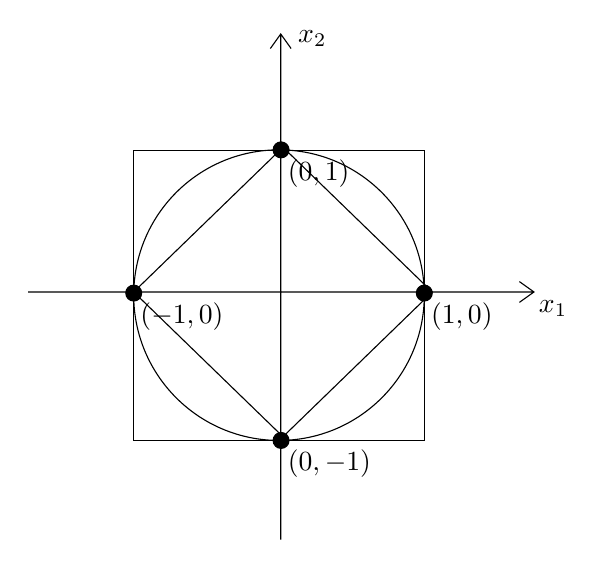
\begin{tikzpicture}[x=0.75pt,y=0.75pt,yscale=-1,xscale=1]
	\draw  (79,159.3) -- (322.65,159.3)(200.65,35) -- (200.65,278.65) (315.65,154.3) -- (322.65,159.3) -- (315.65,164.3) (195.65,42) -- (200.65,35) -- (205.65,42)  ;
	\draw  [fill={rgb, 255:red, 0; green, 0; blue, 0 }  ,fill opacity=1 ] (266,159.82) .. controls (266,157.71) and (267.71,156) .. (269.82,156) .. controls (271.94,156) and (273.65,157.71) .. (273.65,159.82) .. controls (273.65,161.94) and (271.94,163.65) .. (269.82,163.65) .. controls (267.71,163.65) and (266,161.94) .. (266,159.82) -- cycle ;
	\draw  [fill={rgb, 255:red, 0; green, 0; blue, 0 }  ,fill opacity=1 ] (197,90.82) .. controls (197,88.71) and (198.71,87) .. (200.82,87) .. controls (202.94,87) and (204.65,88.71) .. (204.65,90.82) .. controls (204.65,92.94) and (202.94,94.65) .. (200.82,94.65) .. controls (198.71,94.65) and (197,92.94) .. (197,90.82) -- cycle ;
	\draw  [fill={rgb, 255:red, 0; green, 0; blue, 0 }  ,fill opacity=1 ] (126,159.82) .. controls (126,157.71) and (127.71,156) .. (129.82,156) .. controls (131.94,156) and (133.65,157.71) .. (133.65,159.82) .. controls (133.65,161.94) and (131.94,163.65) .. (129.82,163.65) .. controls (127.71,163.65) and (126,161.94) .. (126,159.82) -- cycle ;
	\draw  [fill={rgb, 255:red, 0; green, 0; blue, 0 }  ,fill opacity=1 ] (197,230.82) .. controls (197,228.71) and (198.71,227) .. (200.82,227) .. controls (202.94,227) and (204.65,228.71) .. (204.65,230.82) .. controls (204.65,232.94) and (202.94,234.65) .. (200.82,234.65) .. controls (198.71,234.65) and (197,232.94) .. (197,230.82) -- cycle ;
	\draw   (201.74,89.56) -- (273.65,159.3) -- (201.74,229.04) -- (129.82,159.3) -- cycle ;
	\draw   (129.82,160.82) .. controls (129.82,122.17) and (161.17,90.82) .. (199.82,90.82) .. controls (238.48,90.82) and (269.82,122.17) .. (269.82,160.82) .. controls (269.82,199.48) and (238.48,230.82) .. (199.82,230.82) .. controls (161.17,230.82) and (129.82,199.48) .. (129.82,160.82) -- cycle ;
	\draw   (129.82,91) -- (269.82,91) -- (269.82,230.82) -- (129.82,230.82) -- cycle ;
	\draw (271.82,163.22) node [anchor=north west][inner sep=0.75pt]    {$( 1,0)$};
	\draw (131.82,163.22) node [anchor=north west][inner sep=0.75pt]    {$( -1,0)$};
	\draw (202.82,234.22) node [anchor=north west][inner sep=0.75pt]    {$( 0,-1)$};
	\draw (202.82,94.22) node [anchor=north west][inner sep=0.75pt]    {$( 0,1)$};
	\draw (323.82,162.22) node [anchor=north west][inner sep=0.75pt]    {$x_{1}$};
	\draw (207.82,32.22) node [anchor=north west][inner sep=0.75pt]    {$x_{2}$};
	\end{tikzpicture}	
	\end{center}
\end{eg}
\begin{rmk}
	When solving the regularization problem $\dsst\min_{x\in C}f(x)+\norm{x}^\alpha$, we can choose different types of norms. The shape of the unit ball of the norms will inform which solution is selected. Usually, the solution will be on the boundary of the unit ball. $\l_1$-ball gives sparse solution and using $\l_1$-norm is called the LASSO method. 
\end{rmk}
\begin{df}{Convex Function}
	A function $f:\R^d\to\R$ is called \textit{convex} if $\forall x, y\in\R^d$ and $\lambda\in(0,1)$, we have that $f((1-\lambda)x+\lambda y)\leq(1-\lambda)f(x)+\lambda f(y)$. \textit{Note that this condition is equivalent to saying that $f$ has positive second order derivatives}. 
	\begin{center}
	\tikzset{every picture/.style={line width=0.75pt}}
	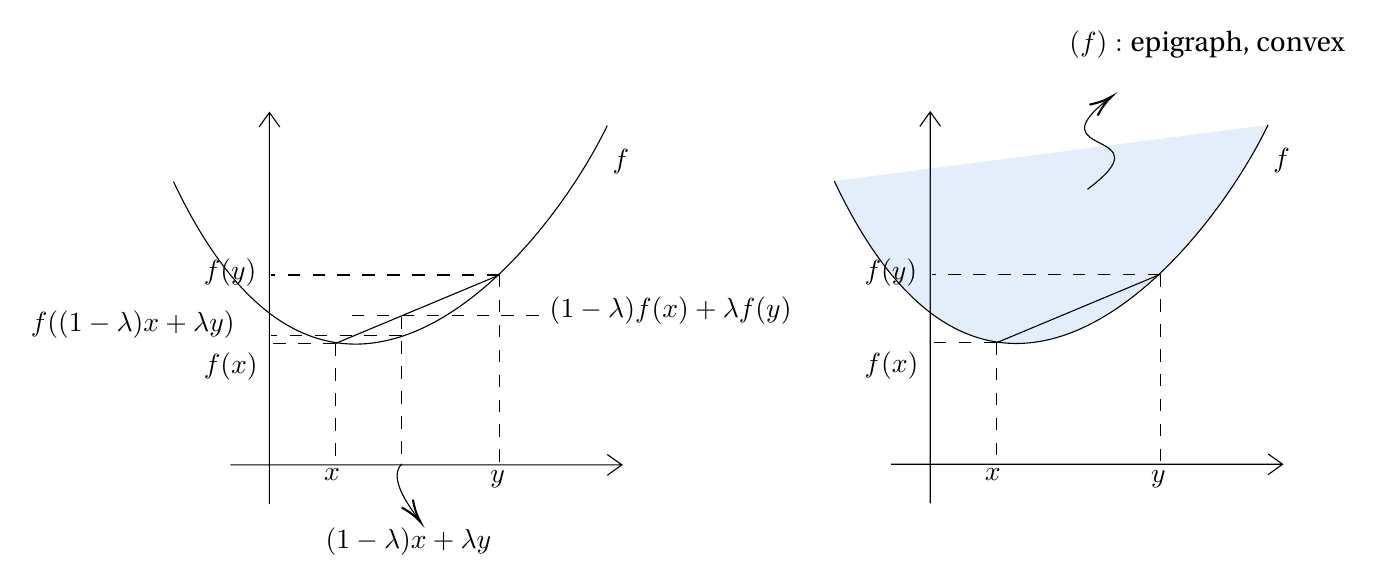
\begin{tikzpicture}[x=0.75pt,y=0.75pt,yscale=-1,xscale=1]
	\draw  (108,231.78) -- (296.65,231.78)(126.86,62) -- (126.86,250.65) (289.65,226.78) -- (296.65,231.78) -- (289.65,236.78) (121.86,69) -- (126.86,62) -- (131.86,69)  ;
	\draw    (80.65,95.3) .. controls (155.65,254.3) and (258.65,132.3) .. (289.65,68.3) ;
	\draw  [dash pattern={on 4.5pt off 4.5pt}]  (158.65,173.3) -- (158.65,231.3) ;
	\draw  [dash pattern={on 4.5pt off 4.5pt}]  (237.65,140.3) -- (237.65,231.3) ;
	\draw  [dash pattern={on 4.5pt off 4.5pt}]  (158.65,173.3) -- (127.65,173.3) ;
	\draw  [dash pattern={on 4.5pt off 4.5pt}]  (237.65,140.3) -- (127.65,140.3) ;
	\draw    (158.65,173.3) -- (237.65,140.3) ;
	\draw  [dash pattern={on 4.5pt off 4.5pt}]  (190.65,160.3) -- (190.65,231.3) ;
	\draw  [dash pattern={on 4.5pt off 4.5pt}]  (190.65,169.3) -- (127.65,169.3) ;
	\draw  [dash pattern={on 4.5pt off 4.5pt}]  (256.65,159.8) -- (166.65,159.8) ;
	\draw    (190.65,231.3) .. controls (184.14,237.81) and (193.2,250.37) .. (198.52,257.73) ;
	\draw [shift={(199.65,259.3)}, rotate = 234.46] [color={rgb, 255:red, 0; green, 0; blue, 0 }  ][line width=0.75]    (10.93,-3.29) .. controls (6.95,-1.4) and (3.31,-0.3) .. (0,0) .. controls (3.31,0.3) and (6.95,1.4) .. (10.93,3.29)   ;
	\draw  (426.35,231.48) -- (615,231.48)(445.22,61.7) -- (445.22,250.35) (608,226.48) -- (615,231.48) -- (608,236.48) (440.22,68.7) -- (445.22,61.7) -- (450.22,68.7)  ;
	\draw [fill={rgb, 255:red, 74; green, 144; blue, 226 }  ,fill opacity=0.15 ]   (399,95) .. controls (474,254) and (577,132) .. (608,68) ;
	\draw  [dash pattern={on 4.5pt off 4.5pt}]  (477,173) -- (477,231) ;
	\draw  [dash pattern={on 4.5pt off 4.5pt}]  (556,140) -- (556,231) ;
	\draw  [dash pattern={on 4.5pt off 4.5pt}]  (477,173) -- (446,173) ;
	\draw  [dash pattern={on 4.5pt off 4.5pt}]  (556,140) -- (446,140) ;
	\draw    (477,173) -- (556,140) ;
	\draw    (521,99) .. controls (560.6,69.3) and (494.01,84) .. (531.48,55.19) ;
	\draw [shift={(532.65,54.3)}, rotate = 143.13] [color={rgb, 255:red, 0; green, 0; blue, 0 }  ][line width=0.75]    (10.93,-3.29) .. controls (6.95,-1.4) and (3.31,-0.3) .. (0,0) .. controls (3.31,0.3) and (6.95,1.4) .. (10.93,3.29)   ;
	\draw (291,78.4) node [anchor=north west][inner sep=0.75pt]    {$f$};
	\draw (152,232.4) node [anchor=north west][inner sep=0.75pt]    {$x$};
	\draw (232,233.4) node [anchor=north west][inner sep=0.75pt]    {$y$};
	\draw (152.65,260.7) node [anchor=north west][inner sep=0.75pt]  [font=\normalsize]  {$( 1-\lambda ) x+\lambda y$};
	\draw (94,176.4) node [anchor=north west][inner sep=0.75pt]    {$f( x)$};
	\draw (10.65,156.4) node [anchor=north west][inner sep=0.75pt]  [font=\normalsize]  {$f(( 1-\lambda ) x+\lambda y)$};
	\draw (260.65,149.4) node [anchor=north west][inner sep=0.75pt]  [font=\normalsize]  {$( 1-\lambda ) f( x) +\lambda f( y)$};
	\draw (94,131.4) node [anchor=north west][inner sep=0.75pt]    {$f( y)$};
	\draw (609.35,78.1) node [anchor=north west][inner sep=0.75pt]    {$f$};
	\draw (470.35,232.1) node [anchor=north west][inner sep=0.75pt]    {$x$};
	\draw (550.35,233.1) node [anchor=north west][inner sep=0.75pt]    {$y$};
	\draw (412.35,176.1) node [anchor=north west][inner sep=0.75pt]    {$f( x)$};
	\draw (412.35,131.1) node [anchor=north west][inner sep=0.75pt]    {$f( y)$};
	\draw (511,21.4) node [anchor=north west][inner sep=0.75pt]    {$\epi( f) :\text{epigraph, convex}$};
	\end{tikzpicture}
	\end{center}
\end{df}
\begin{rmk}
	The definition of a convex function is to say that the graph of the function is below the straight line of connecting any two points on the graph. 	
\end{rmk}
\begin{df}{Epigraph of $f$}
	Define $\epi(f)\coloneqq\qty{(x,z)\in\R^{d+1}:z\geq f(x)}$. \textit{Note that ``epi'' means ``up'' in greek.}	
\end{df}
\begin{thm}{Duality of Convexity}
	A function $f:\R^d\to\R$ is convex if and only if $\epi(f)$ is convex.	
\end{thm}
\begin{eg}{A Nonexample}
	\begin{center}
	\tikzset{every picture/.style={line width=0.75pt}}
	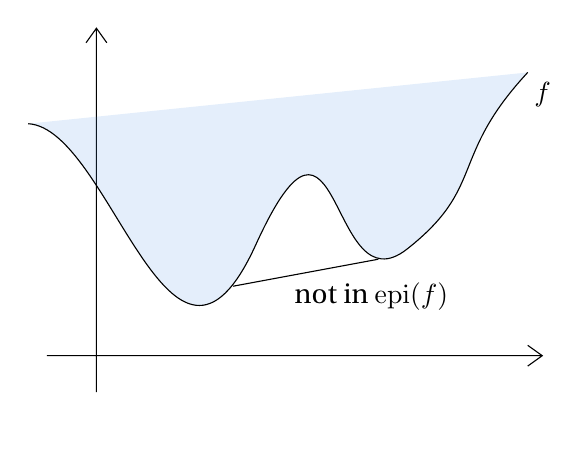
\begin{tikzpicture}[x=0.75pt,y=0.75pt,yscale=-1,xscale=1]
	\draw  (50,227.77) -- (288.65,227.77)(73.86,70) -- (73.86,245.3) (281.65,222.77) -- (288.65,227.77) -- (281.65,232.77) (68.86,77) -- (73.86,70) -- (78.86,77)  ;
	\draw [fill={rgb, 255:red, 74; green, 144; blue, 226 }  ,fill opacity=0.15 ]   (41,116) .. controls (80.65,118.3) and (109.65,264.3) .. (150.65,174.3) .. controls (191.65,84.3) and (185.65,206.3) .. (223.65,176.3) .. controls (261.65,146.3) and (243.65,132.3) .. (281.65,91.3) ;
	\draw    (139.65,194.3) -- (209.65,181.3) ;
	\draw (283.65,94.7) node [anchor=north west][inner sep=0.75pt]    {$f$};
	\draw (168,191.4) node [anchor=north west][inner sep=0.75pt]    {$\text{not in} \ \mathrm{epi}( f)$};
	\end{tikzpicture}
	\end{center}	
\end{eg}
\begin{prf}
	($\Rightarrow$) Suppose $f$ is convex. Let $(x,z),(y,w)\in\epi(f)$ and $\lambda\in(0,1)$. Our goal is to show that $(1-\lambda)(x,z)+\lambda(y,w)\in\epi(f)$ as well. Note that \[(1-\lambda)(x,z)+\lambda(y,w)=((1-\lambda)x+\lambda y, (1-\lambda)x+\lambda w).\] Since $(x,z),(y,w)\in\epi(f)$, we have $z\geq f(x)$ and $w\geq f(y)$. Therefore \begin{align*}(1-\lambda)z+\lambda w&\geq(1-\lambda)f(x)+\lambda f(y)\\&\geq f((1-\lambda)x+\lambda y)&by\ convexity\ of\ f\pqde
	\end{align*}\par 
	($\Leftarrow$) Suppose $\epi(f)$ is a convex set. Note that $\forall x,y\in\R^d$, by definition of $\epi(f)$, we have $(x,f(x))\in\epi(f)$ and $(y,f(y))\in\epi(f)$. Then, by convexity, we know \[(1-\lambda)(x,f(x))+\lambda(y,f(y))=((1-\lambda)x+\lambda y,(1-\lambda)f(x)+\lambda f(y))\in\epi(f).\] Again, by definition of $\epi(f)$, we have \[f((1-\lambda)x+\lambda y)\leq(1-\lambda)f(x)+\lambda f(y).\] Therefore, $f$ is convex. 
\end{prf}
\begin{df}{$\alpha$-Level Set}
	Let $f:\R^d\to\R$ be an arbitrary function and $\alpha\in\R$. Then, the \textit{$\alpha$-level set} of $f$ is $\Lev(f,\alpha)\coloneqq\qty{x:\in\R^d:f(x)\leq\alpha}$. 
\end{df}
\begin{center}
\tikzset{every picture/.style={line width=0.75pt}}
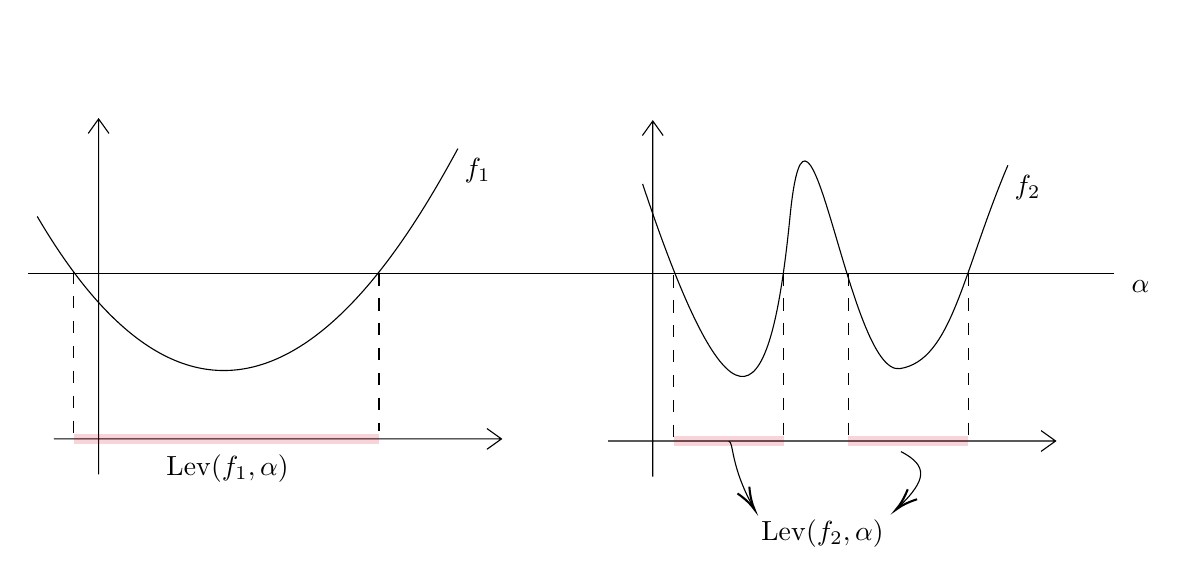
\begin{tikzpicture}[x=0.75pt,y=0.75pt,yscale=-1,xscale=1]
\draw  (50,209.17) -- (265.65,209.17)(71.56,55) -- (71.56,226.3) (258.65,204.17) -- (265.65,209.17) -- (258.65,214.17) (66.56,62) -- (71.56,55) -- (76.56,62)  ;
\draw  (317,210.17) -- (532.65,210.17)(338.56,56) -- (338.56,227.3) (525.65,205.17) -- (532.65,210.17) -- (525.65,215.17) (333.56,63) -- (338.56,56) -- (343.56,63)  ;
\draw    (42,102) .. controls (133.65,258.3) and (212.65,128.3) .. (244.65,69.3) ;
\draw    (333.65,86.3) .. controls (378.65,221.3) and (395.65,193.3) .. (404.65,102.3) .. controls (413.65,11.3) and (432.65,179.3) .. (457.65,175.3) .. controls (482.65,171.3) and (487.65,129.3) .. (509.65,77.3) ;
\draw    (37.65,129.3) -- (560.65,129.3) ;
\draw  [dash pattern={on 4.5pt off 4.5pt}]  (59.65,128.3) -- (59.65,210.3) ;
\draw  [dash pattern={on 4.5pt off 4.5pt}]  (206.65,129.3) -- (206.65,205.3) ;
\draw  [dash pattern={on 4.5pt off 4.5pt}]  (348.65,130.3) -- (348.65,212.3) ;
\draw  [dash pattern={on 4.5pt off 4.5pt}]  (401.65,129.3) -- (401.65,211.3) ;
\draw  [dash pattern={on 4.5pt off 4.5pt}]  (432.65,129.3) -- (432.65,211.3) ;
\draw  [dash pattern={on 4.5pt off 4.5pt}]  (490.65,129.3) -- (490.65,211.3) ;
\draw [color={rgb, 255:red, 208; green, 2; blue, 27 }  ,draw opacity=0.17 ][fill={rgb, 255:red, 208; green, 2; blue, 27 }  ,fill opacity=0.28 ][line width=3.75]    (59.65,209.3) -- (206.65,209.3) ;
\draw [color={rgb, 255:red, 208; green, 2; blue, 27 }  ,draw opacity=0.17 ][fill={rgb, 255:red, 208; green, 2; blue, 27 }  ,fill opacity=0.28 ][line width=3.75]    (348.65,210.3) -- (401.65,210.3) ;
\draw [color={rgb, 255:red, 208; green, 2; blue, 27 }  ,draw opacity=0.17 ][fill={rgb, 255:red, 208; green, 2; blue, 27 }  ,fill opacity=0.28 ][line width=3.75]    (432.65,210.3) -- (490.65,210.3) ;
\draw    (375.15,210.3) .. controls (377.59,210.3) and (375.75,221.71) .. (386.78,241.74) ;
\draw [shift={(387.65,243.3)}, rotate = 240.26] [color={rgb, 255:red, 0; green, 0; blue, 0 }  ][line width=0.75]    (10.93,-3.29) .. controls (6.95,-1.4) and (3.31,-0.3) .. (0,0) .. controls (3.31,0.3) and (6.95,1.4) .. (10.93,3.29)   ;
\draw    (458.15,215.3) .. controls (471.24,222.09) and (470.7,228.88) .. (456.96,242.06) ;
\draw [shift={(455.65,243.3)}, rotate = 316.97] [color={rgb, 255:red, 0; green, 0; blue, 0 }  ][line width=0.75]    (10.93,-3.29) .. controls (6.95,-1.4) and (3.31,-0.3) .. (0,0) .. controls (3.31,0.3) and (6.95,1.4) .. (10.93,3.29)   ;
\draw (568,131.4) node [anchor=north west][inner sep=0.75pt]    {$\alpha $};
\draw (246.65,72.7) node [anchor=north west][inner sep=0.75pt]    {$f_{1}$};
\draw (511.65,80.7) node [anchor=north west][inner sep=0.75pt]    {$f_{2}$};
\draw (103,215.4) node [anchor=north west][inner sep=0.75pt]    {$\mathrm{Lev}( f_{1} ,\alpha )$};
\draw (389.65,246.7) node [anchor=north west][inner sep=0.75pt]    {$\mathrm{Lev}( f_{2} ,\alpha )$};
\end{tikzpicture}
\end{center}
\begin{thm}{}
	If $f$ is convex, then $\Lev(f,\alpha)$ are convex $\forall\ \alpha\in\R$.
\end{thm}
\begin{rmk}
	By convention, we consider empty set as convex as well	
\end{rmk}
\begin{prf}
	Let $x,y\in\Lev(f,\alpha)$ and $\lambda\in(0,1)$. \par \textit{WTS: $(1-\lambda)x+\lambda y\in\Lev(f,\alpha)\quad\Longleftarrow\quad f((1-\lambda)x+\lambda y)\leq\alpha$}.\par As $x,y\in\Lev(f,\alpha)$, then $f(x)\leq\alpha$ and $f(y)\leq\alpha$. So, \[(1-\lambda)f(x)+\lambda f(y)\leq (1-\lambda)\alpha+\lambda\alpha=\alpha.\] By convexity of $f$, we know \[f((1-\lambda)x+\lambda y)\leq(1-\lambda)f(x)+\lambda f(y)\leq\alpha.\] So, $(1-\lambda)x+\lambda y\in\Lev(f,\alpha)$.
\end{prf}
\begin{rmk}
	Often, we have $\dsst\min_{f(x)\leq\alpha}g(x)$. In this case, $C=\qty{x:f(x)\leq\alpha}=\Lev(f,\alpha)$. In fact, every $\Lev(f,\alpha)$ is corresponding to a certain convex function. Therefore, Theorem 4.1.10 can be strengthen into an if-and-only-if statement.
\end{rmk}
\begin{eg}{Example 4.1.3 Revisit}
	Consider $B_r(x_0)=\qty{x\in\R^d:\norm{x-x_0}\leq r}$. If $f(x)=\norm{x-x_0}$, $x\in\R^d$, then $B_r(x_0)=\Lev(f,r)$. Show that $B_r(x_0)$ is convex. 
	\begin{prf}
		To prove the statement, we first consider the convexity of $f(x)$: 
		\begin{clm*}
			$f$ is convex.
		\end{clm*}
		\begin{proof}\textit{
			Let $x,y\in\R^d$ and $\lambda\in(0,1)$. WTS: $\norm{(1-\lambda)x+\lambda y}\leq(1-\lambda)\norm{x}+\lambda\norm{y}$.\newline Note that \begin{align*}
			\norm{(1-\lambda)x+\lambda y}&\leq\norm{(1-\lambda)x}+\norm{\lambda y}&triangular\ inequality\\&=(1-\lambda)\norm{x}+\lambda\norm{y}&homogeneity\end{align*} So, $f$ is convex.} 
		\end{proof}
		As $f$ is convex and $B_r(x_0)=\Lev(f,r)$, by Theorem 4.1.10, $B_r(x_0)$ is convex. 
	\end{prf}
\end{eg}
\begin{rmk}
	Example 4.1.11 offers another approach to prove a set is convex other than applying the definition: proving it is the level set of a convex function. This is a more powerful approach and can be applied into different types of questions.
\end{rmk}
\begin{thm}{Operations Preserving Convexity I}
	Assume that $f_1,f_2,\dots,f_p$ are convex functions. Then, 
	\begin{enumerate}
		\item $\alpha_1f_1+\alpha_2f_2+\cdots+\alpha_pf_p$ is convex $\forall\ \alpha_1,\dots,\alpha_p\geq0$.
		\item $f(x)=\max\qty{f_1(x),f_2(x),\dots,f_p(x)}$ is a convex function.
	\end{enumerate}	
\end{thm}
\begin{prf}
	Here, we will offer a proof of Theorem 4.1.12 (2). Let $x,y\in\R^d$ and $\lambda\in(0,1)$. \textit{We want to show $f((1-\lambda)x+\lambda y)\leq(1-\lambda)f(x)+\lambda f(y)$.} Note that \begin{align*}f_i((1-\lambda)x+\lambda y)&\leq(1-\lambda)f_i(x)+\lambda f_i(y)&convexity\ of\ f_i\\&\leq(1-\lambda)f(x)+\lambda f(x),\quad\forall\ i&definition\ of\ f: f_i(x)\leq f(x)\end{align*} So, \[\max_if_i((1-\lambda)x+\lambda y)\leq(1-\lambda)f(x)+\lambda f(x).\] By definition of $f$, that is, $f((1-\lambda)x+\lambda y)\leq(1-\lambda)f(x)+\lambda f(y)$.
\end{prf}
\begin{thm}{Operations Preserving Convexity II}
	Let $f$ be a convex function. Then, $g(y)=f(Ay+b)$ is also convex, where $A$ is a matrix and $b$ is a vector. 	
\end{thm}
\begin{prf}
	Let $y,z\in\dom(g)$, the domain of $g$. Then, \begin{align*}g((1-\lambda)y+\lambda z)&=f(A((1-\lambda)y+\lambda z)+b)\\&=f((1-\lambda)Ay+\lambda Az+(1-\lambda)b+\lambda b)&linearity\ of\ A\\&=f((1-\lambda)(Ay+b)+\lambda(Az+b))\\&\leq(1-\lambda)f(Ay+b)+\lambda f(Az+b)&convexity\ of\ f\\&=(1-\lambda)g(y)+\lambda g(z)&definition\ of\ g\end{align*} As $g((1-\lambda)y+\lambda z)\leq(1-\lambda)g(y)+\lambda g(z)$, $g$ is convex. 
\end{prf}
\begin{thm}{Operations Preserving Convexity III}
	Assume $f:\R^d\to\R$ is convex and $g:\R\to\R$ is an increasing convex function. Then, $h(x)=(g\circ f)(x)=g(f(x))$ is also convex.
\end{thm}
\begin{prf}
	Let $x,y\in\R^d$ and $\lambda\in(0,1)$. Then, by the convexity of $f$, we have \[f((1-\lambda)x+\lambda y)\leq(1-\lambda)f(x)+\lambda f(y).\] Further, due to $g$ being monotonically increasing, \[g(f((1-\lambda)x+\lambda y))\leq g((1-\lambda)f(x)+\lambda f(y)).\] Therefore, \begin{align*}h((1-\lambda)x+\lambda y)=g(f((1-\lambda)x+\lambda y))&\leq g((1-\lambda)f(x)+\lambda f(y))\\&\leq (1-\lambda)g(f(x))+\lambda g(f(y))&convexity\ of\ g\\&=(1-\lambda)h(x)+\lambda h(y)& definition\ of\ h\end{align*} As $h((1-\lambda)x+\lambda y)\leq(1-\lambda)h(x)+\lambda h(y)$, $h$ is convex.
\end{prf}
\begin{clm}
	Let $C_1,C_2,\dots,C_p$ be convex sets. Then, $C=\dsst\bigcap_{i=1}^p=C_1\cap C_2\cap\cdots\cap C_p$ is also convex. 
\end{clm}
\begin{rmk}
	The union of convex sets, $C=\dsst\bigcup_{i=1}^pC_i=C_1\cup C_2\cup\cdots\cup C_p$	might not be a convex set. 
\end{rmk}
\begin{cor}{}
	Let $f_1,f_2,\dots,f_p$ be convex functions and $\alpha_1,\alpha_2,\dots,\alpha_p\in\R$. Then, \begin{align*}C&=\qty{x:f_1(x)\leq\alpha_1,f_2(x)\leq\alpha_2,\dots,f_p(x)\leq\alpha_p}\\&=\Lev(f_1,\alpha_1)\cap\Lev(f_2,\alpha_2)\cap\cdots\cap\Lev(f_p,\alpha_p)\\&=\bigcap_{i=1}^p\Lev(f_i,\alpha_i)\end{align*} is also convex.
\end{cor}
\begin{rmk}
	Consider an optimization problem $\dsst\min_{\substack{f_1(x)\leq\alpha_1\\f_2(x)\leq\alpha_2\\\cdots\\f_p(x)\leq\alpha_p}}g(x)$. If $f_i$ are convex, then the constrain set of this problem is also convex as a result of Corollary 4.1.16.
\end{rmk}




\end{document}